\documentclass{jsarticle}

\usepackage{ascmac}
\usepackage{color}
\usepackage{url}
\usepackage{moreverb}
\usepackage{here}
\usepackage[dvipdfmx]{graphicx}
\usepackage[margin=20mm]{geometry}
\usepackage{float}


\begin{document}

\title{Beam Deflection Simulator Explanation}
\author{日本語}
\maketitle
\newpage

\tableofcontents

\newpage

\part{操作案内}
ここでは, シミュレータの使い方について説明する.

\newpage
\section{梁の設定}

\begin{figure}[H]
\begin{center}
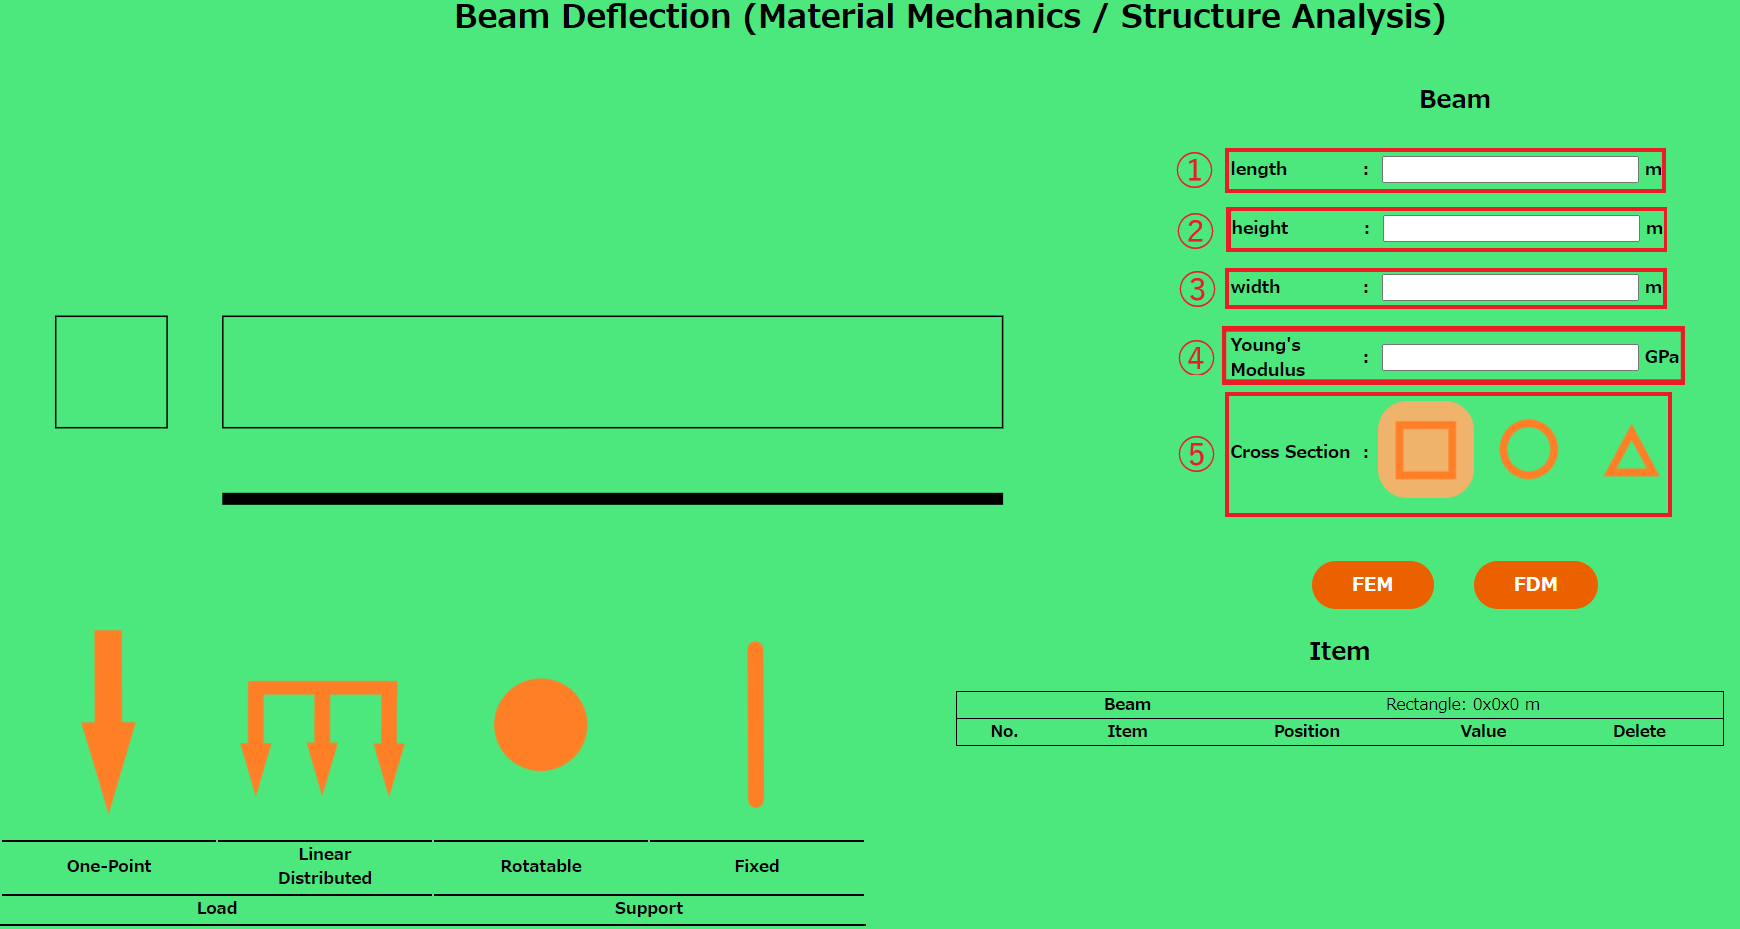
\includegraphics[width=15cm]{Beam_Setting.png}
\caption{梁の設定画面}
\end{center}
\end{figure}

梁については,
\begin{itemize}
\item[\textcircled{\scriptsize 1}] 梁の長さ (length)
\item[\textcircled{\scriptsize 2}] 梁の高さ (height)
\item[\textcircled{\scriptsize 3}] 梁の幅 (width)
\item[\textcircled{\scriptsize 4}] 梁のヤング率 (Young's Modulus)
\item[\textcircled{\scriptsize 5}] 断面形状 (Cross Section)
\end{itemize}
を設定することができる. 各変数がさす部位については, 記入欄をクリックすることによって左上の図に描画される. このシミュレーターでは, 梁の材質や形状の変化を記述することはできず, 一様な梁のみを対象としている.

なお, 梁の長さが設定されていない場合, 荷重や支持店の設定移ることはできない.


\newpage
\section{支持点の設定}
\subsection{回転支持点 Rotatable Support}
このシミュレータにおいて, 回転支持点は, ローラー$\bigcirc$及びピン$\bigtriangleup$に対応する.
\begin{figure}[H]
\begin{center}
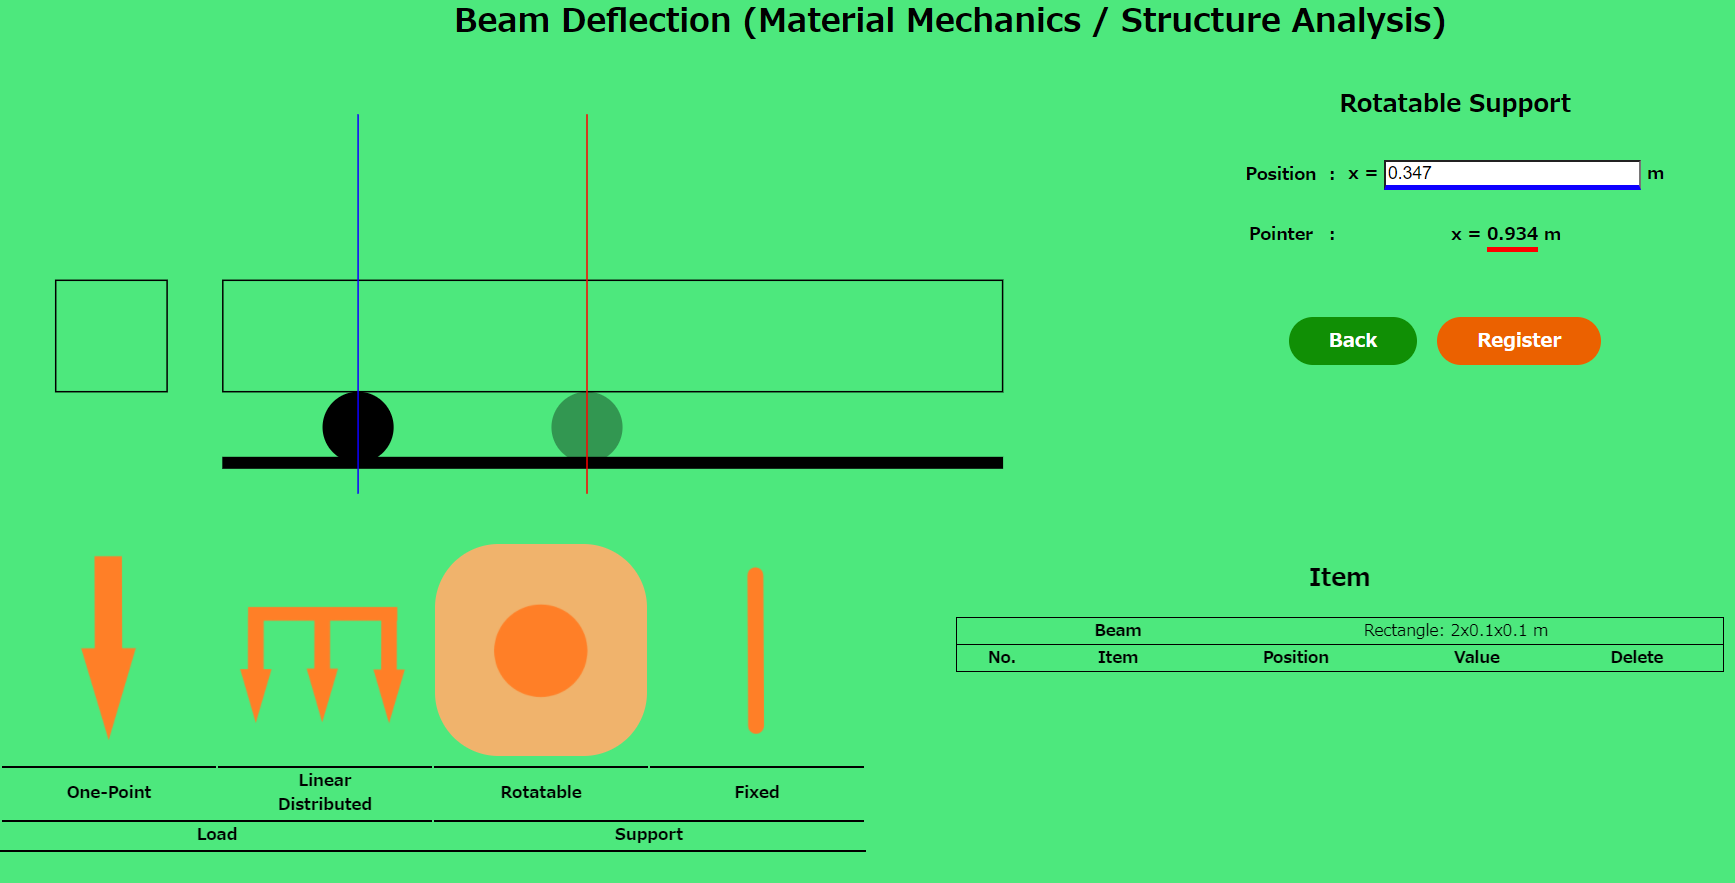
\includegraphics[width=15cm]{Rotatable_Support_Setting.png}
\caption{回転支持点の設定画面}
\end{center}
\end{figure}
回転支持点の設定では, その位置を設定することができる. 数値入力と図におけるクリック入力に対応している. 

図では, \textcolor{blue}{青線が現在設定されている位置}, \textcolor{red}{赤線が現在のポインタの位置}を示している. 設定後は, [Resister]を押すことにより設定が完了する.

\newpage
\subsection{固定支持点 Fixed Support}
このシミュレータにおいて, 固定支持点は固定端に対応する.
\begin{figure}[H]
\begin{center}
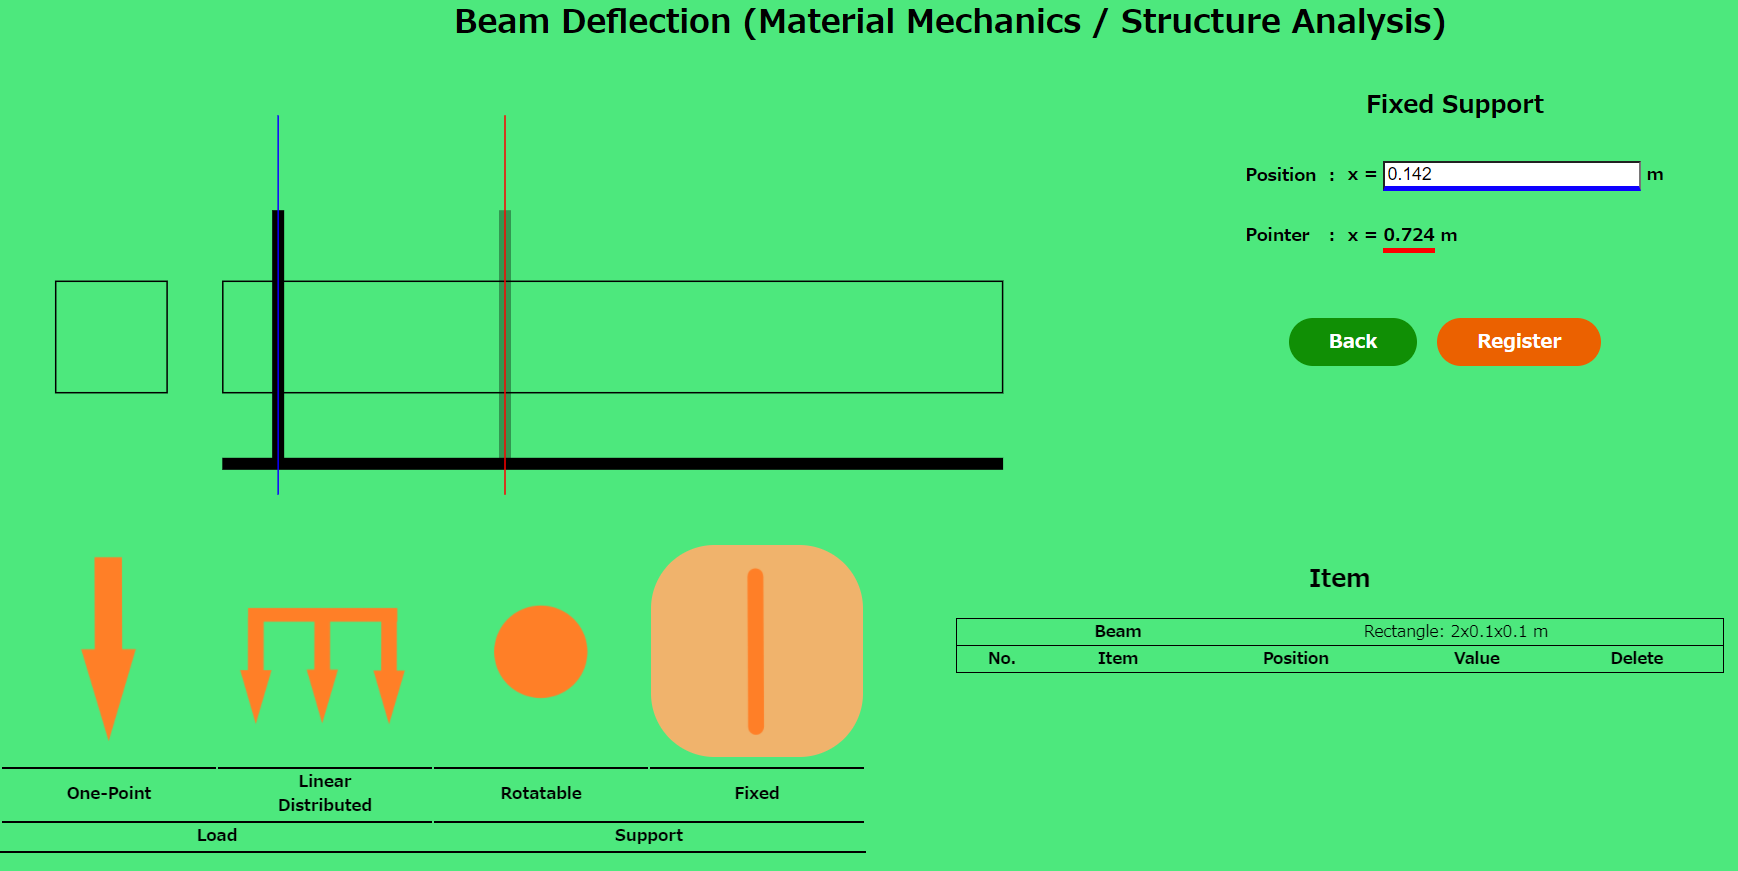
\includegraphics[width=15cm]{Fixed_Support_Setting.png}
\caption{固定支持点の設定画面}
\end{center}
\end{figure}
設定については, 回転支持点と全く同じである.

\newpage
\section{荷重の設定}
\subsection{一点荷重 One-Point Load}
\begin{figure}[H]
\begin{center}
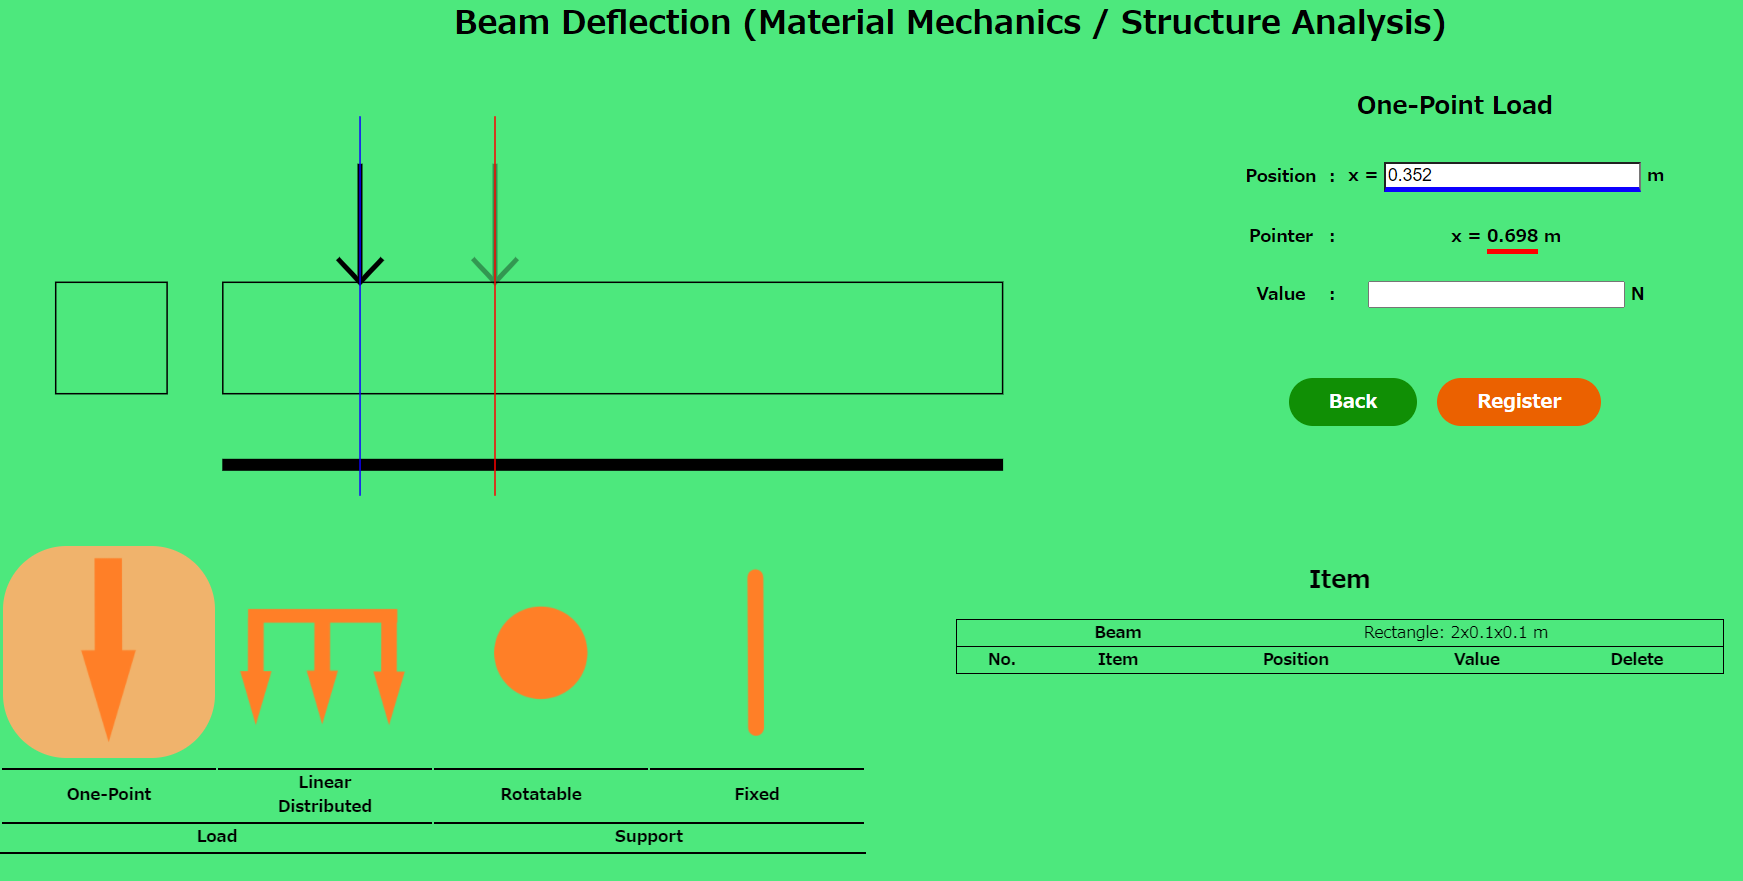
\includegraphics[width=15cm]{One-Point_Load_Setting.png}
\caption{一点荷重の設定画面}
\end{center}
\end{figure}

一点荷重の設定では, 荷重が加わる点とその大きさを設定できる. 大きさは数値入力のみに対応しており, 荷重の位置は数値及びクリック入力に対応している. 図では, \textcolor{blue}{青線が現在設定されている位置}, \textcolor{red}{赤線が現在のポインタの位置}を示している. 設定後は, [Resister]を押すことにより設定が完了する.

\newpage
\subsection{線形分布荷重 Linear Distributed Load}
\begin{figure}[H]
\begin{center}
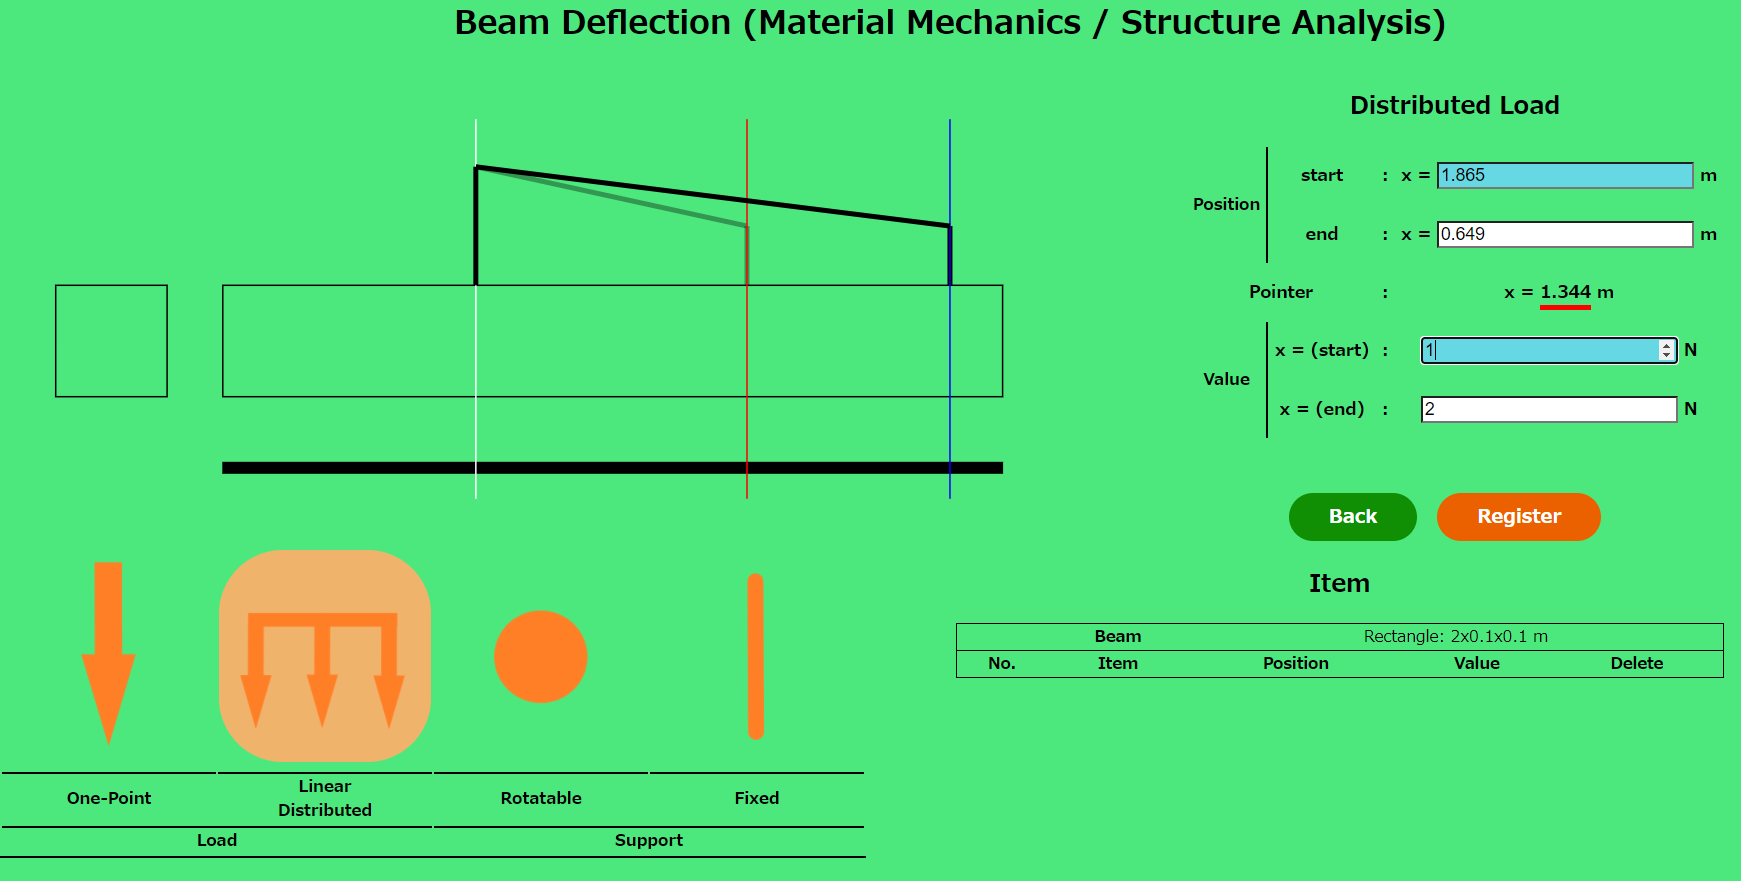
\includegraphics[width=15cm]{Distributed_Load_Setting.png}
\caption{線形分布荷重の設定画面}
\end{center}
\end{figure}

線形分布荷重の設定では, 特定の2点の位置とそれぞれにおける荷重の大きさを設定することで, 線形の分布荷重を設定する(このシミュレータでは, 2次以上の高次関数や指数関数, 三角関数に従う分布荷重には対応していません). 数値入力欄の背景が青色の部分がクリック入力に対応しています. また端点での荷重の設定は, 一点荷重と同じである. 

\section{数値計算手法と結果}
設定した, 支持点や荷重は左下にリストとして表示される. そして, FEMやFDMの手法を選択することで, シミュレーションを開始する. 結果では, 
\begin{itemize}
\item \textcolor{green}{たわみ (Deflection)}
\item たわみ角 (Slope)
\item \textcolor{red}{曲げモーメント (Bending Moment)}
\item \textcolor{cyan}{剪断力 (Shear Force)}
\end{itemize}
がグラフとして作成されるとともに, たわみの様子が描画される. 

また, 同様の状況を異なる手法により解析をすることも可能である.


\newpage

\part{数値計算理論}
ここでは, このソフトウェアで使われている2つの数値解析手法,
\begin{itemize}
\item FEM (有限要素法)
\item FDM (有限差分法)
\end{itemize}
について, 説明する. 
\newpage

\section{仮定}
このシミュレータによる計算では, 計算及びモデルの単純化のために, 以下を仮定する.
\begin{itemize}
\item この梁の材質と断面形状は均一である.
\item この梁のたわみは1次元上での計算結果を表示し, 横にずれることはないものとする.
\item 梁自体の重さは考慮しない
\end{itemize}


\section{原理}
\subsection{オイラーの梁理論}
このシミュレータにおいては, 大学の材料力学で学習した, オイラーの理論に基づいて, 以下を支配方程式とする.
\begin{eqnarray}
EI\frac{d^4w}{dx^4} &=& -q
\end{eqnarray}
\begin{center}
($E$: ヤング率 [Pa], $I$: 断面二次モーメント [m$^4$], $w$: たわみ [m], $q$: 与えられる外力 [N])
\end{center}

後述をするが, 今回のシミュレーションにおいて以下のデータを入力する必要がある.
\begin{itemize}
\item 外力 $q$ (FEM, FDM)
\item 両端における剪断力 $V$ (FEM)
\item 両端における曲げモーメント $M$ (FEM)
\end{itemize}

外力には支持力も含まれるため, 静定梁問題においては力のつり合いとモーメントのつり合いから支持力を算出する必要がある. また, 不静定梁では外力を求めることができない. そこで有効な手段はFDMである. 後述するようにFDMでは支持力を入力する必要がないため, 入力されたデータのみから不静定梁のたわみのシミュレーションを行うことができる. 逆に\underline{FEMでは, 端に支持点がある場合, 不静定梁の適切なたわみを計算することができない場合がある}.

\subsection{FEM 有限要素法}
\subsubsection{弱形式}
前項で求めた支配方程式を変形した場合,
\begin{eqnarray*}
\frac{d^2\mbox{\boldmath $M$}}{dx^2}=-q
\end{eqnarray*}
となる. これを弱形式に変換する. 部分積分を行い,
\begin{eqnarray*}
\int^{x_b}_{x_a}\mbox{\boldmath $B$}^TEI\mbox{\boldmath $B$}\mbox{\boldmath $U$}dx&=&\left[\mbox{\boldmath $N$}^T\mbox{\boldmath $V$}\right]^{x_b}_{x_a}-\left[\frac{d\mbox{\boldmath $N$}^T}{dx}\mbox{\boldmath $M$}\right]^{x_b}_{x_a}+\int^{x_b}_{x_a}\mbox{\boldmath $N$}^Tqdx
\end{eqnarray*}
\begin{center}
$\left(\mbox{\boldmath $B$}=\frac{d^2\mbox{\boldmath $N$}}{dx^2}\right)$
\end{center}
となる弱形式が得られる.

\subsubsection{ガラーキン有限要素法}
弱形式を行列形式にする. ここで,
\begin{eqnarray*}
\mbox{\boldmath $K$}\mbox{\boldmath $U$}=\mbox{\boldmath $f$}_b+\mbox{\boldmath $f$}_l
\end{eqnarray*}
とおくと,
\begin{eqnarray*}
\mbox{\boldmath $K$} &=& \int^{x_b}_{x_a}\mbox{\boldmath $B$}^TEI\mbox{\boldmath $B$}dx \\
\mbox{\boldmath $f$}_b &=& \left[\mbox{\boldmath $N$}^T\mbox{\boldmath $V$}\right]^{x_b}_{x_a}-\left[\frac{d\mbox{\boldmath $N$}^T}{dx}\mbox{\boldmath $M$}\right]^{x_b}_{x_a} \\
\mbox{\boldmath $f$}_l &=& \int^{x_b}_{x_a}\mbox{\boldmath $N$}^Tqdx
\end{eqnarray*}
となる. 今回は1次元熱伝導問題や1次元弾性問題とは異なり, 支配方程式の微分が2階であるため, 区分的関数を用いることができない. そこで, 以下を形状関数とする.
\begin{eqnarray*}
N_1 &=& 1-3\frac{x^2}{L^2}+2\frac{x^3}{L^3} \\
N_2 &=& -x\left(1-2\frac{x}{L}+\frac{x^2}{L^2}\right) \\
N_3 &=& \frac{x^2}{L^2}\left(3-2\frac{x}{L}\right) \\
N_4 &=& -\frac{x^2}{L}\left(\frac{x}{L}-1\right)
\end{eqnarray*}
\begin{figure}[H]
\begin{center}
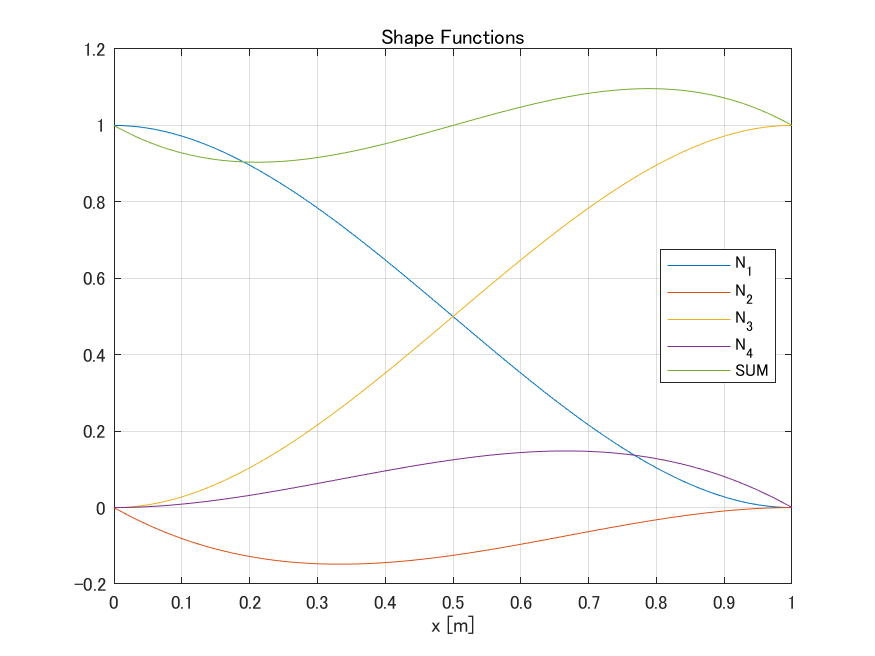
\includegraphics[width=10cm]{Shape_Functions.png}
\caption{FEA 形状関数}
\end{center}
\end{figure}

これを用いると, 弾性力学の考え方より$\mbox{\boldmath $K$}$および, $\mbox{\boldmath $f$}_b$が以下のように決まる.
\renewcommand{\arraystretch}{1.3}
\begin{eqnarray*}
\mbox{\boldmath $K$} &=& \left[
\begin{array}{cccc}
\frac{12EI}{L^3} & -\frac{6EI}{L^2} & -\frac{12EI}{L^3} & -\frac{6EI}{L^2} \\
-\frac{6EI}{L^2} & \frac{4EI}{L} & \frac{6EI}{L^2} & \frac{2EI}{L} \\
-\frac{12EI}{L^3} & \frac{6EI}{L^2} & \frac{12EI}{L^3} & \frac{6EI}{L^2} \\
-\frac{6EI}{L^2} & \frac{2EI}{L} & \frac{6EI}{L^2} & \frac{4EI}{L}
\end{array}\right] \\
\mbox{\boldmath $f$}_b &=& \left[
\begin{array}{c}
-V_{x=x_a} \\
M_{x=x_a} \\
V_{x=x_b} \\
-M_{x=x_b}
\end{array}\right]
\end{eqnarray*}


\subsection{FDM 有限差分法}
支配方程式において, $EI$が均一であることを仮定して, 微分を差分近似すると,
\begin{eqnarray}
EI\frac{w_{i+2}-4w_{i+1}+6w_i-4w_{i-1}+w_{i-2}}{(\Delta x)^4} = -q
\end{eqnarray}
これを行列形式に変換することで,各点でのたわみをシミュレーションすることができる. さらに支配方程式の微分を中央差分スキームにより近似することによって, 以下のように, たわみ角$\theta$, 曲げモーメント$M$, 剪断力$V$が求まる.
\begin{eqnarray*}
\theta_i &=& \frac{w_{i+1}-w_{i-1}}{2(\Delta x)} \\
M_i &=& -EI\frac{\theta_{i+1}-\theta_{i-1}}{2(\Delta x)} \\
V_i &=& \frac{M_{i+1}-M_{i-1}}{2(\Delta x)}
\end{eqnarray*}
しかし, この方法では, 主に梁の端の部分と支持点における誤差が顕著にみられる. これは, その点での各値が連続ではないことに由来する. そこで, このシミュレータでは, 剪断力が解析的に求められる静定梁問題では, 解析的に求めることができる解析解を表示している.

\subsection{境界条件}
今回は, FEMやFDMを用いて, 微分方程式を線形連立方程式に変換してシミュレーションを行う. しかし, FEMやFDMで作られる行列は特異であり, そのままでは解くことができない. そこで, 境界条件を入力することで, たわみを解く. 入力されたデータに基づいて, 以下を境界条件として入力する.
\begin{table}[H]
\begin{center}
\caption{境界条件}
\begin{tabular}{|c|c|}
\hline
支持形態 & 境界条件 \\
\hline
Rotatable Support & $w = 0$ \\
\hline
Fixed Support & $w = 0$, $\theta = 0$ \\
\hline
\end{tabular}
\end{center}
\end{table}

また, コード単純化のため, $x=x_i$での境界条件は,
\begin{eqnarray*}
K[i][i] &=& K[i][i]\times10^{15} \\
f[i] &=& 0
\end{eqnarray*}
と入力する. これにより, 境界条件の入力を単純化することができる.

\newpage

\part{シミュレーション (静定梁問題)}
ここからは, 実際にこのソフトウェアの計算により得られるシミュレーション結果を表示する. 最初に, 解析解を容易に得ることができる, 静定梁問題を題材として, 解析解とシミュレーション結果を比較する.

シミュレータでは, 100要素有限要素解析及び201節点有限差分解析を行っている.

\newpage

\section{両端支持梁}
\subsection{一点荷重}
\subsubsection{モデル}
\begin{figure}[H]
\begin{center}
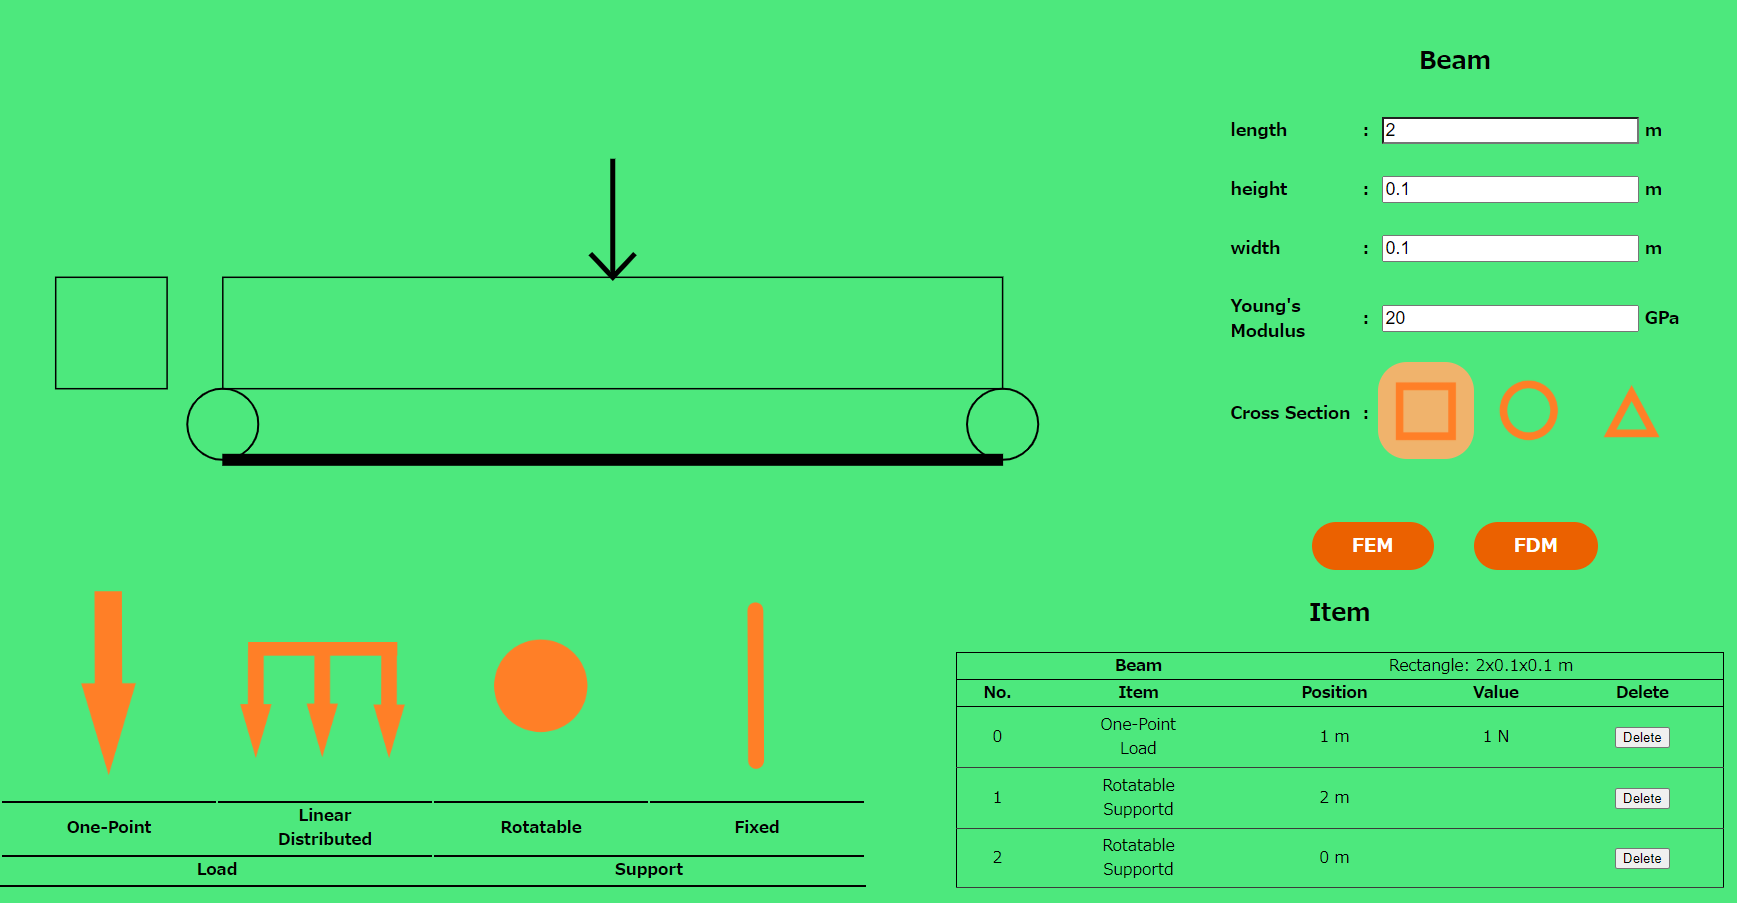
\includegraphics[width=13cm]{simple_one_model.PNG}
\caption{両端支持梁 一点荷重モデル}
\end{center}
\end{figure}

\subsubsection{解析解}

\begin{eqnarray*}
V &=& \left\{ \begin{array}{ll}
    -\frac{W}{2} & (0\leq x<\frac{l}{2}) \\
    \frac{W}{2} & (\frac{l}{2}\leq x < l)
  \end{array} \right. \\
M &=& \left\{ \begin{array}{ll}
    -\frac{W}{2}x & (0\leq x<\frac{l}{2}) \\
    \frac{W}{2}(x-l) & (\frac{l}{2}\leq x < l)
  \end{array} \right. \\
\theta &=& \left\{ \begin{array}{ll}
    \frac{W}{2EI}\left(\frac{x^2}{2}-\frac{l^3}{8}\right) & (0\leq x<\frac{l}{2}) \\
    -\frac{W}{2EI}\left(\frac{x^2}{2}-lx+\frac{3}{8}l^2\right) & (\frac{l}{2}\leq x < l)
  \end{array} \right. \\
w &=& \left\{ \begin{array}{ll}
    \frac{W}{2EI}\left(\frac{x^3}{6}-\frac{l^3}{8}x\right) & (0\leq x<\frac{l}{2}) \\
    -\frac{W}{2EI}\left(\frac{x^3}{6}-\frac{l}{2}x^2+\frac{3}{8}l^2x-\frac{l^3}{24}\right) & (\frac{l}{2}\leq x < l)
  \end{array} \right.
\end{eqnarray*}

今回はモデルに示されているように, $l=2$ [m], $W=1$ [N], $E=20$ [GPa], $I=8.33\times10^{-6}$ [m$^4$]を用いる. これらの値を代入することで得られる解析解は以下のようになる(MATLABによる計算).

\begin{figure}[H]
\begin{center}
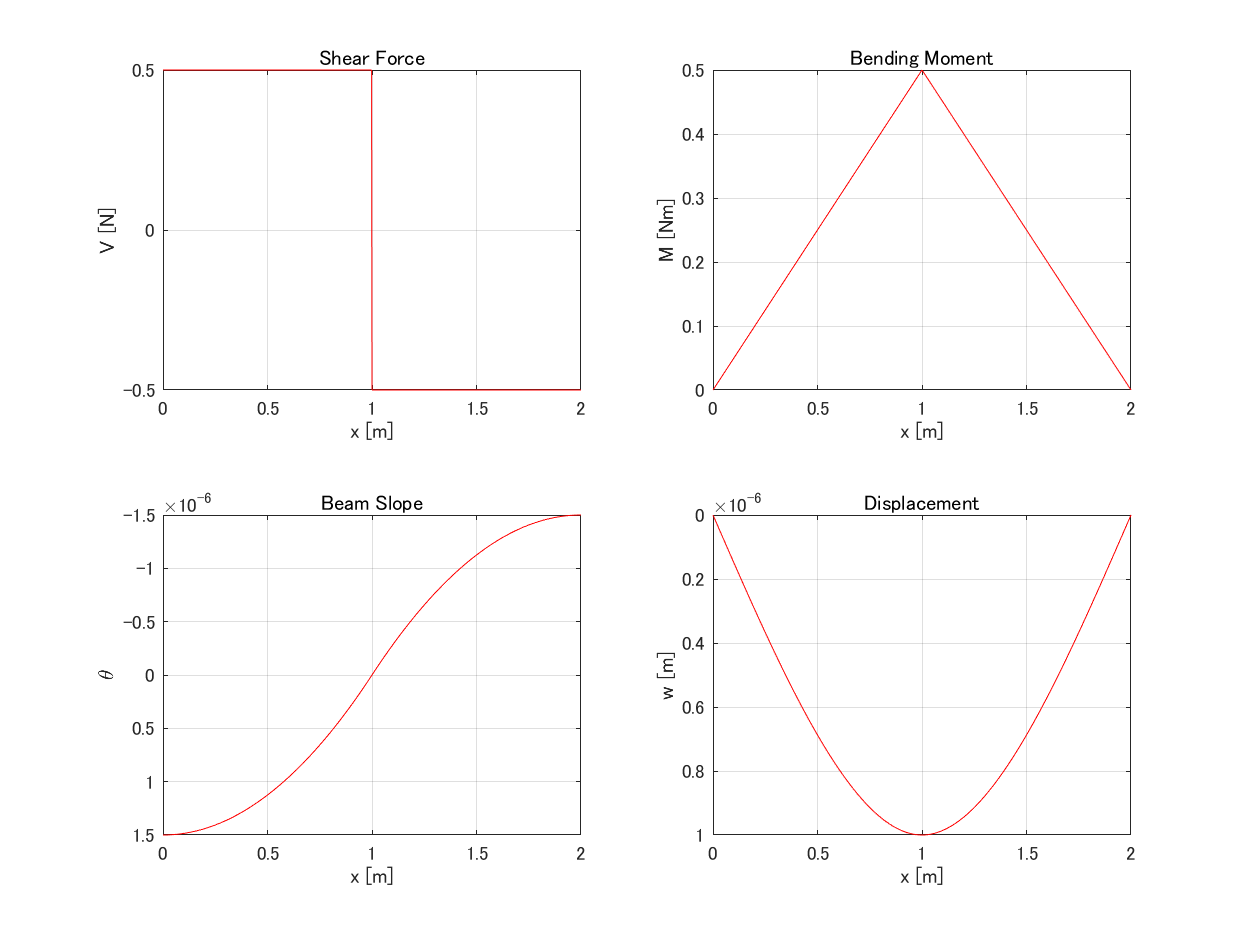
\includegraphics[width=10cm]{Simple_Supported_Beam.png}
\caption{両端支持梁 一点荷重 解析解}
\end{center}
\end{figure}

\subsubsection{シミュレーション結果}
\begin{table}[H]
\begin{center}
\caption{両端支持梁 一点荷重モデル シミュレーション結果の比較}
\begin{tabular}{|c|c|c|}
\hline
 & FEM & FDM \\
\hline
\hline
$V$ &
\begin{minipage}{6truecm}
\centering
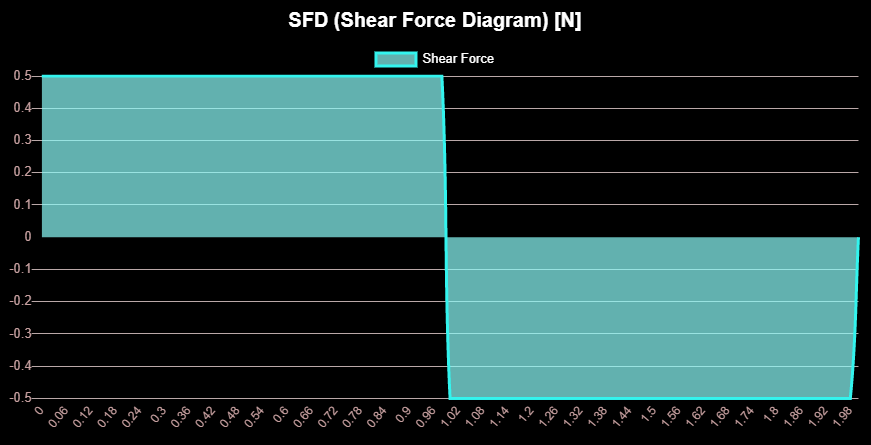
\includegraphics[width=6truecm]{simple_one_model_FEM_sf.PNG}
\end{minipage}
&
\begin{minipage}{6truecm}
\centering
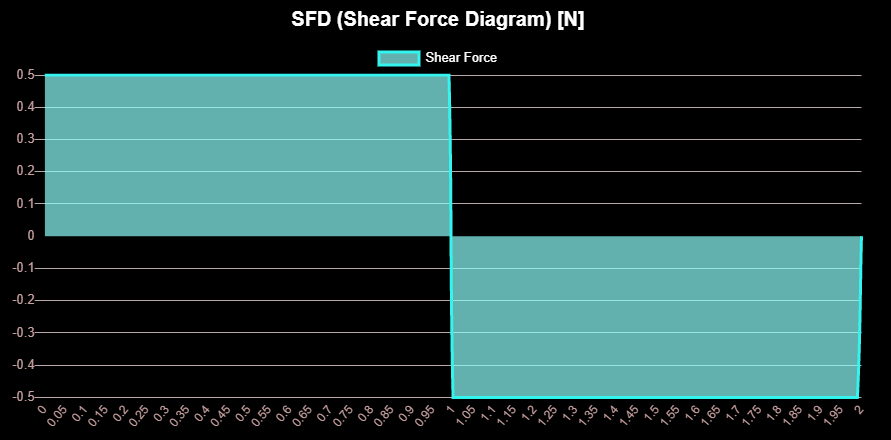
\includegraphics[width=6truecm]{simple_one_model_FDM_sf.PNG}
\end{minipage}
\\
\hline
$M$ &
\begin{minipage}{6truecm}
\centering
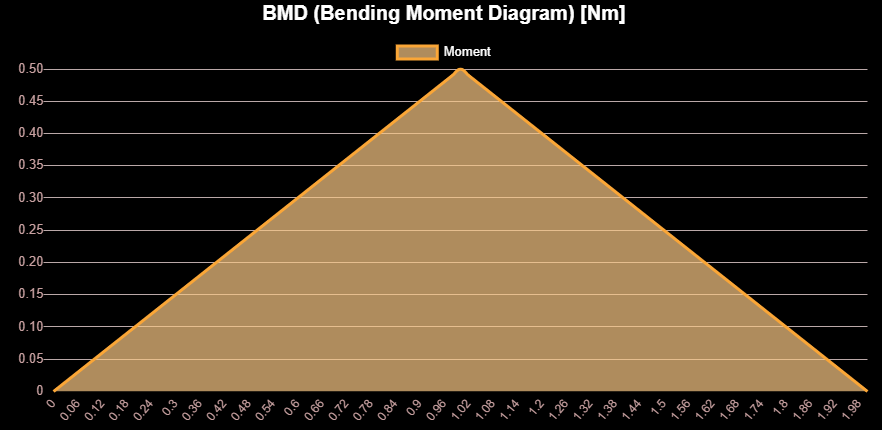
\includegraphics[width=6cm]{simple_one_model_FEM_bm.PNG}
\end{minipage}
&
\begin{minipage}{6truecm}
\centering
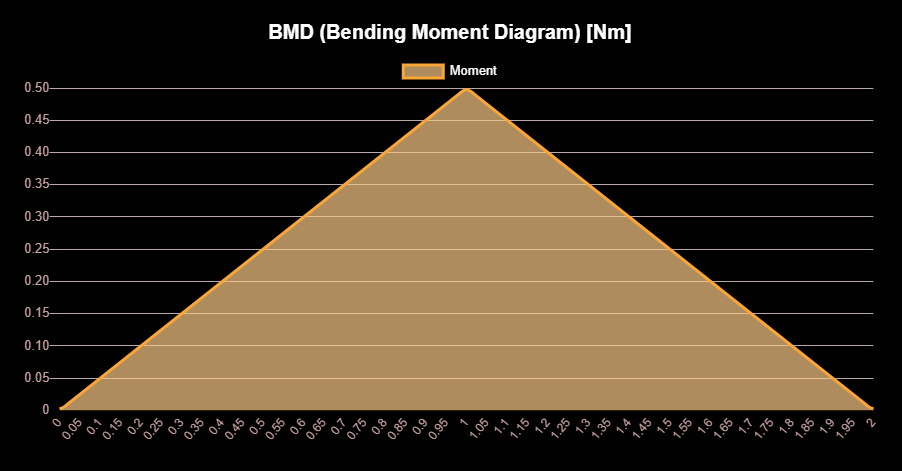
\includegraphics[width=6cm]{simple_one_model_FDM_bm.PNG}
\end{minipage}
\\
\hline
$\theta$ &
\begin{minipage}{6truecm}
\centering
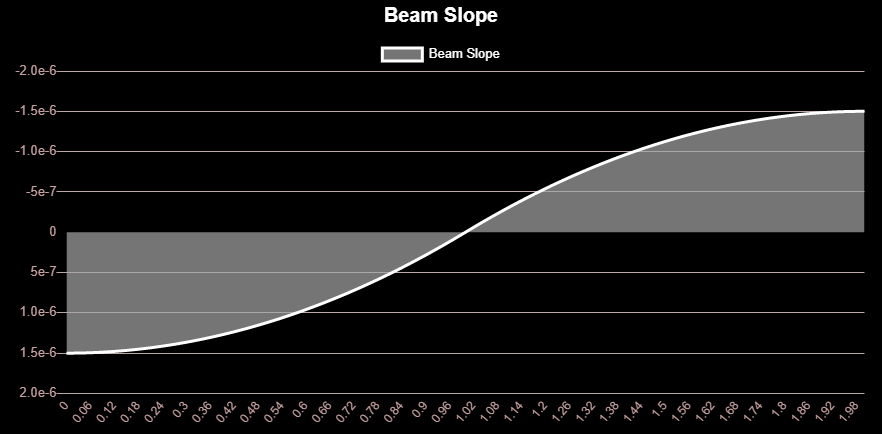
\includegraphics[width=6cm]{simple_one_model_FEM_slo.PNG}
\end{minipage}
&
\begin{minipage}{6truecm}
\centering
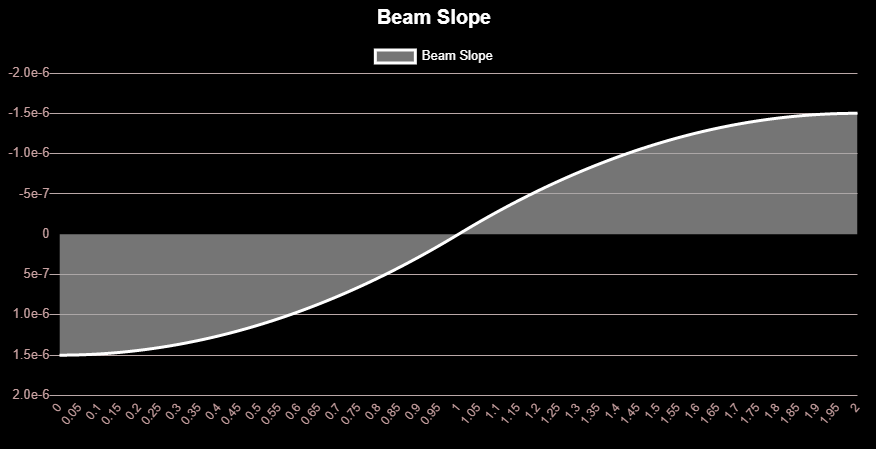
\includegraphics[width=6cm]{simple_one_model_FDM_slo.PNG}
\end{minipage}
\\
\hline
$w$ &
\begin{minipage}{6truecm}
\centering
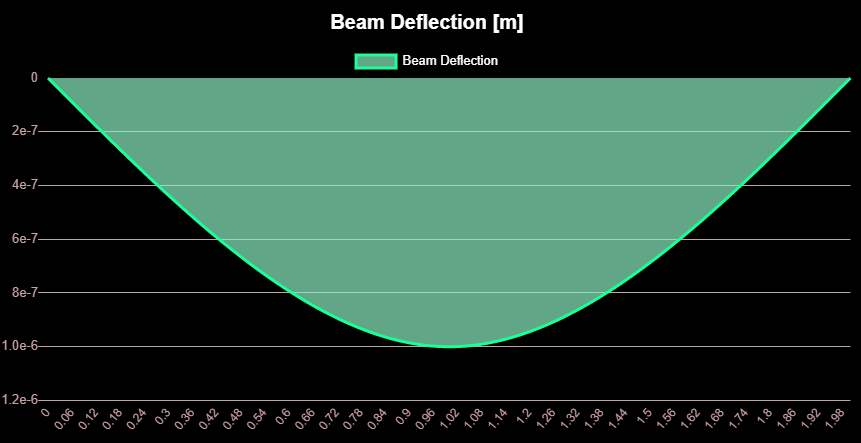
\includegraphics[width=6cm]{simple_one_model_FEM_def.PNG}
\end{minipage}
&
\begin{minipage}{6truecm}
\centering
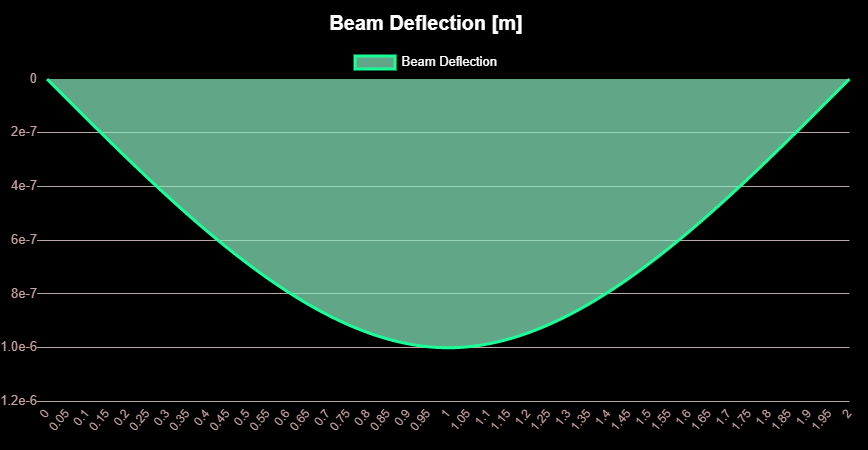
\includegraphics[width=6cm]{simple_one_model_FDM_def.PNG}
\end{minipage}
\\
\hline
\end{tabular}
\end{center}
\end{table}

\newpage
\subsection{分布荷重}
\subsubsection{モデル}
\begin{figure}[H]
\begin{center}
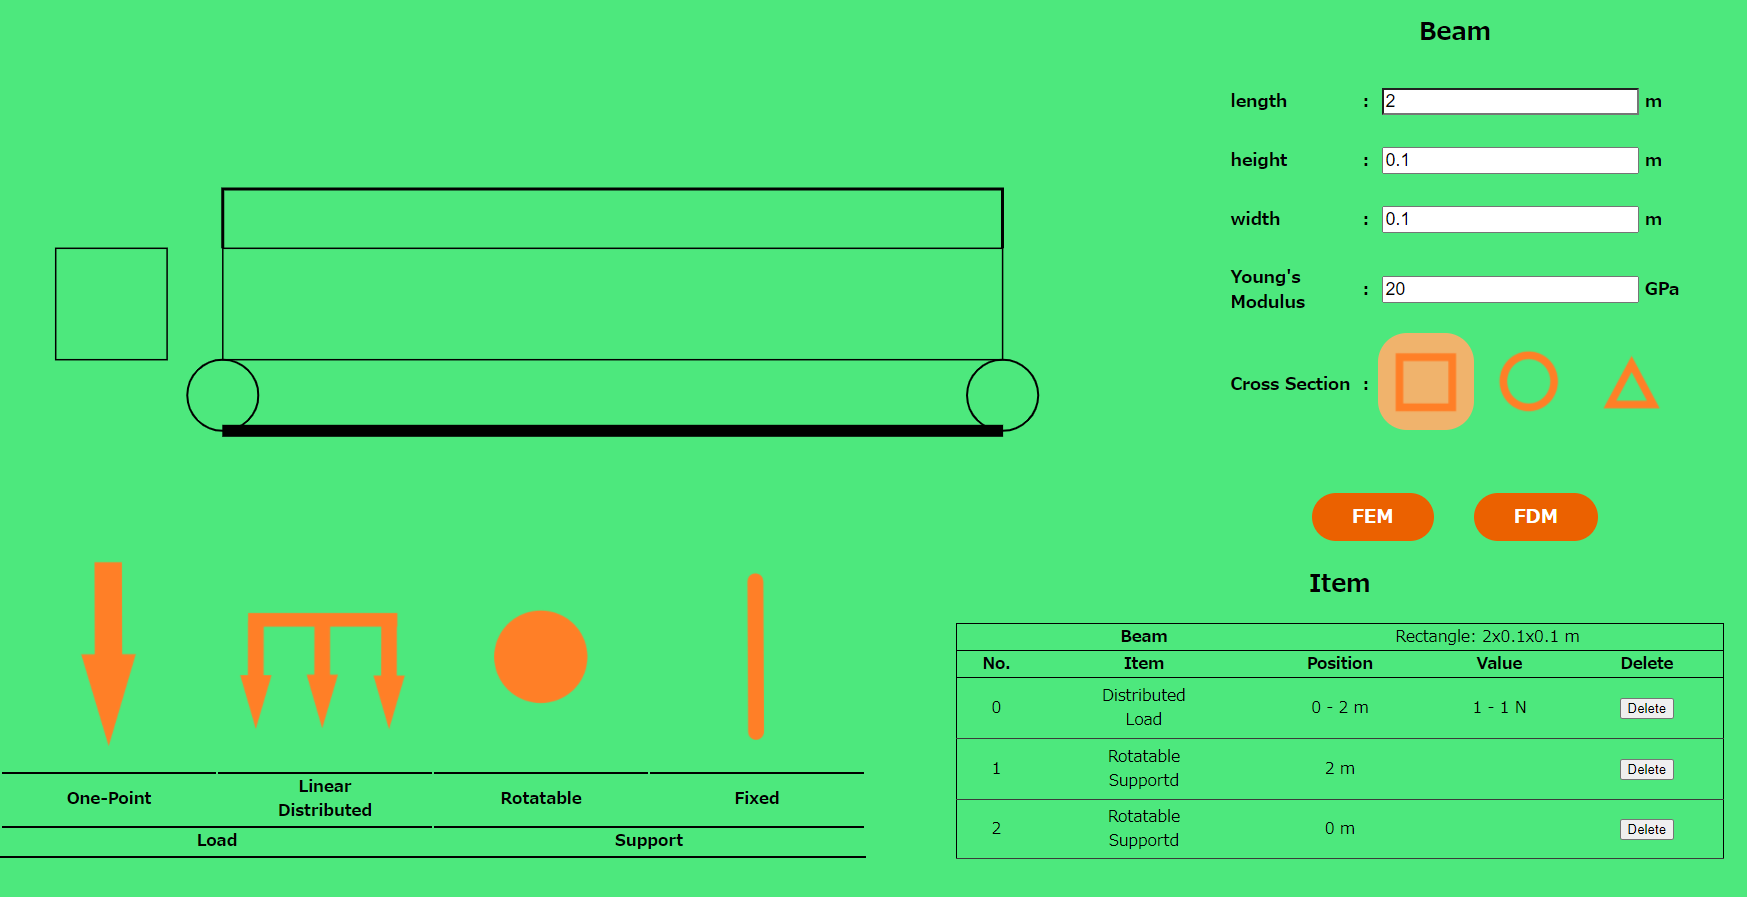
\includegraphics[width=13cm]{simple_distributed_model.PNG}
\caption{両端支持梁 分布荷重モデル}
\end{center}
\end{figure}

\subsubsection{解析解}

\begin{eqnarray*}
V &=& \frac{lx}{2}-Wx \\
M &=& \frac{W}{2}(lx-x^2) \\
\theta &=& -\frac{W}{2EI}\left(-\frac{x^3}{3}+\frac{l}{2}x^2-\frac{l^3}{12}\right) \\
w &=& -\frac{W}{2EI}\left(-\frac{x^4}{12}+\frac{l}{6}x^3-\frac{l^3}{12}x\right)
\end{eqnarray*}
今回もモデルに示されているように, $l=2$ [m], $W=1$ [N], $E=20$ [GPa], $I=8.33\times10^{-6}$ [m$^4$]を用いる. これらの値を代入することで得られる解析解は以下のようになる(MATLABによる計算).

\begin{figure}[H]
\begin{center}
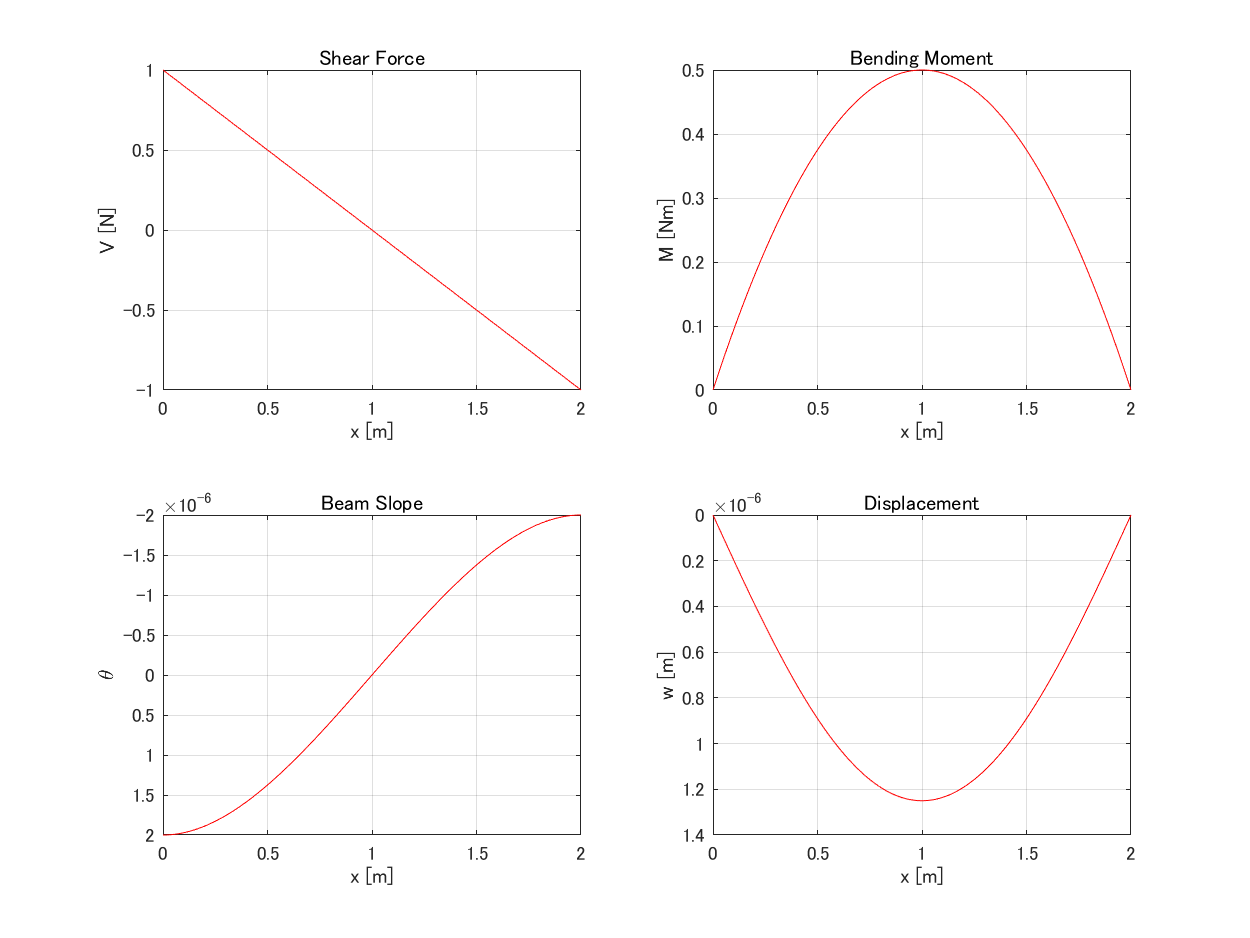
\includegraphics[width=10cm]{Simple_Supported_Distributed_Beam.png}
\caption{両端支持梁 分布荷重 解析解}
\end{center}
\end{figure}

\subsubsection{シミュレーション結果}
\begin{table}[H]
\begin{center}
\caption{両端支持梁 分布荷重モデル シミュレーション結果の比較}
\begin{tabular}{|c|c|c|}
\hline
 & FEM & FDM \\
\hline
\hline
$V$ &
\begin{minipage}{6truecm}
\centering
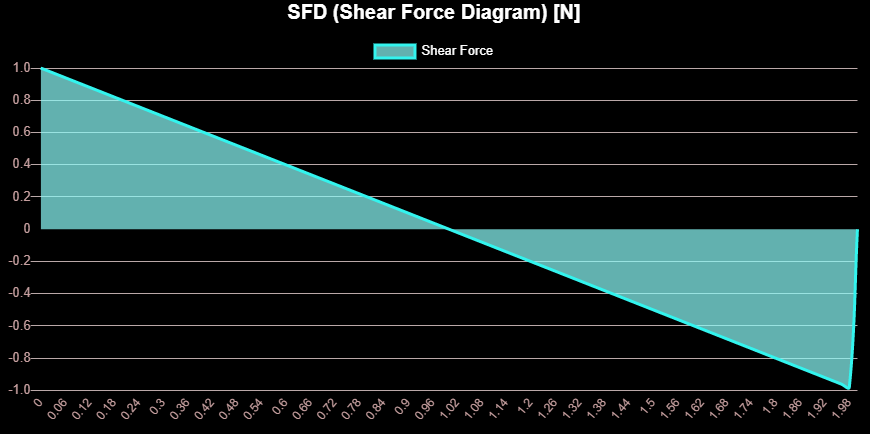
\includegraphics[width=6truecm]{simple_distributed_model_FEM_sf.PNG}
\end{minipage}
&
\begin{minipage}{6truecm}
\centering
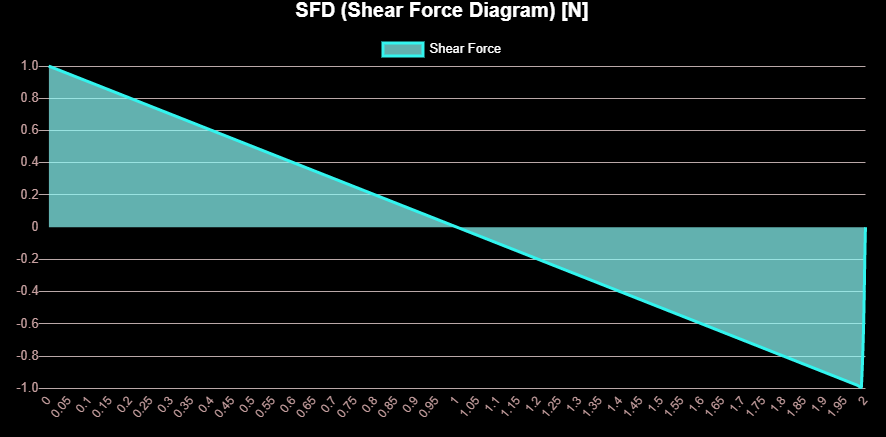
\includegraphics[width=6truecm]{simple_distributed_model_FDM_sf.PNG}
\end{minipage}
\\
\hline
$M$ &
\begin{minipage}{6truecm}
\centering
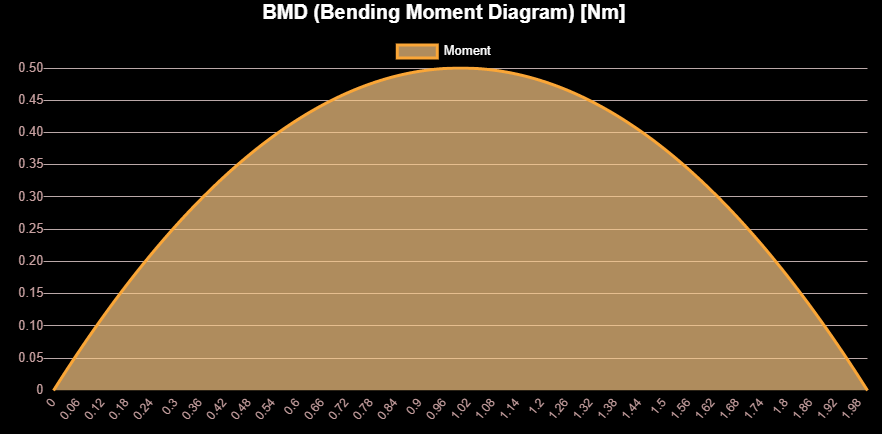
\includegraphics[width=6cm]{simple_distributed_model_FEM_bm.PNG}
\end{minipage}
&
\begin{minipage}{6truecm}
\centering
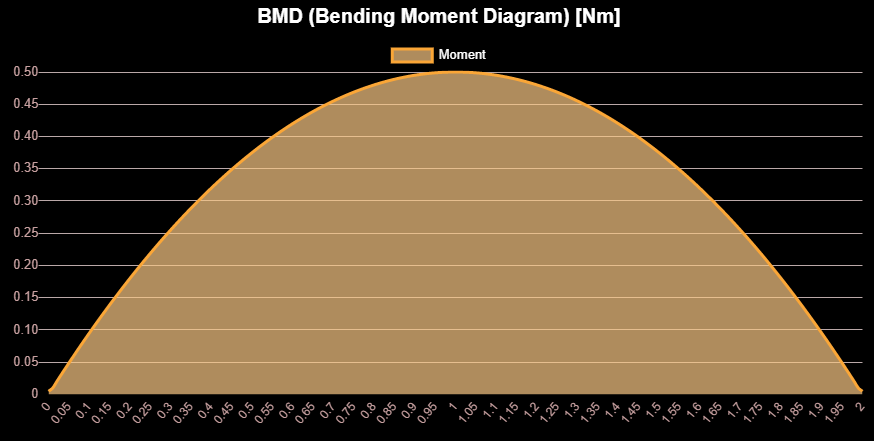
\includegraphics[width=6cm]{simple_distributed_model_FDM_bm.PNG}
\end{minipage}
\\
\hline
$\theta$ &
\begin{minipage}{6truecm}
\centering
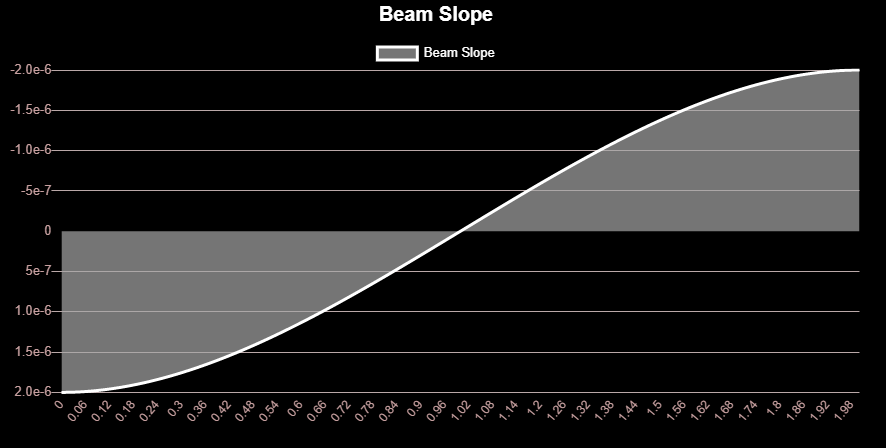
\includegraphics[width=6cm]{simple_distributed_model_FEM_slo.PNG}
\end{minipage}
&
\begin{minipage}{6truecm}
\centering
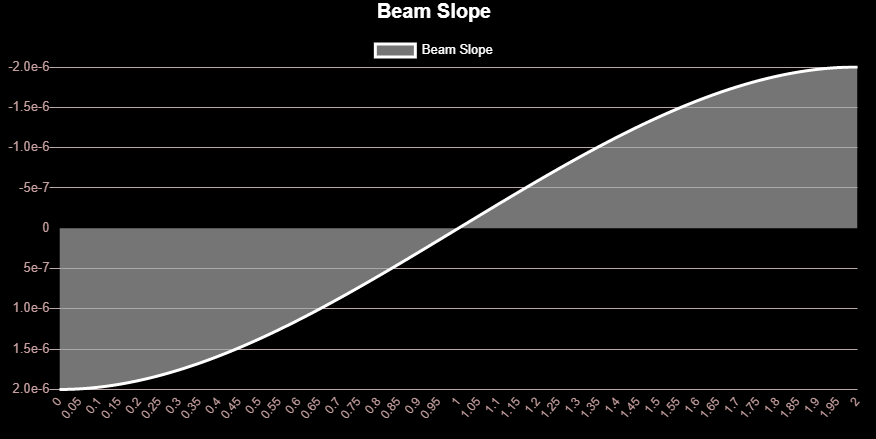
\includegraphics[width=6cm]{simple_distributed_model_FDM_slo.PNG}
\end{minipage}
\\
\hline
$w$ &
\begin{minipage}{6truecm}
\centering
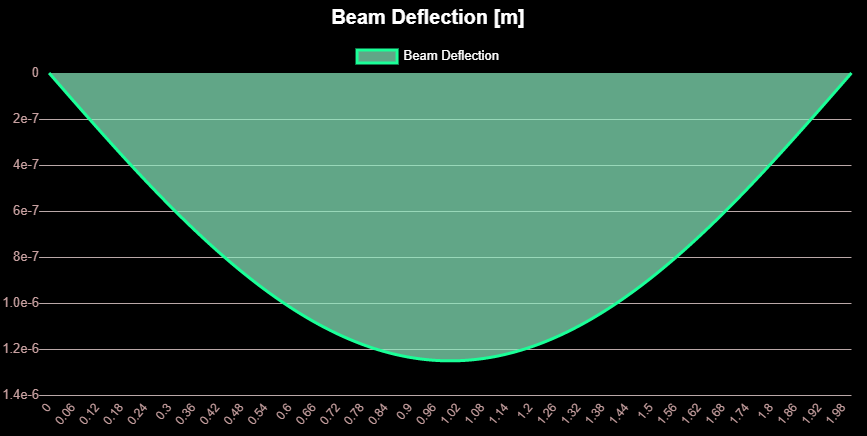
\includegraphics[width=6cm]{simple_distributed_model_FEM_def.PNG}
\end{minipage}
&
\begin{minipage}{6truecm}
\centering
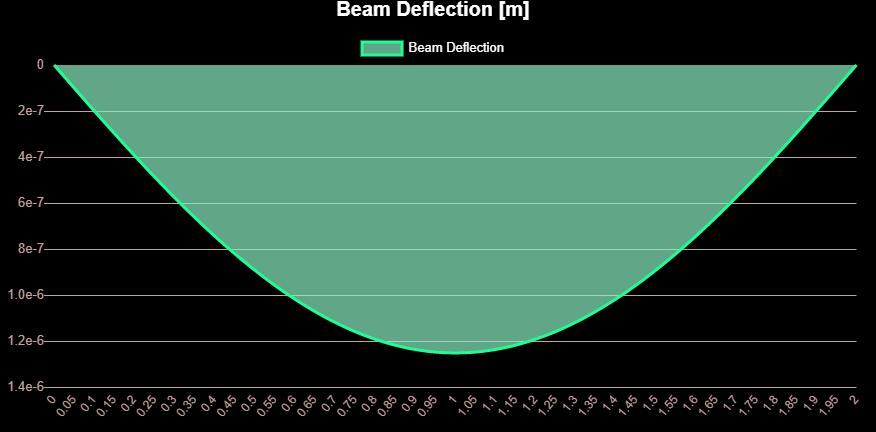
\includegraphics[width=6cm]{simple_distributed_model_FDM_def.PNG}
\end{minipage}
\\
\hline
\end{tabular}
\end{center}
\end{table}

\newpage
\section{片持ち梁}
\subsection{一点荷重}
\subsubsection{モデル}

\begin{figure}[H]
\begin{center}
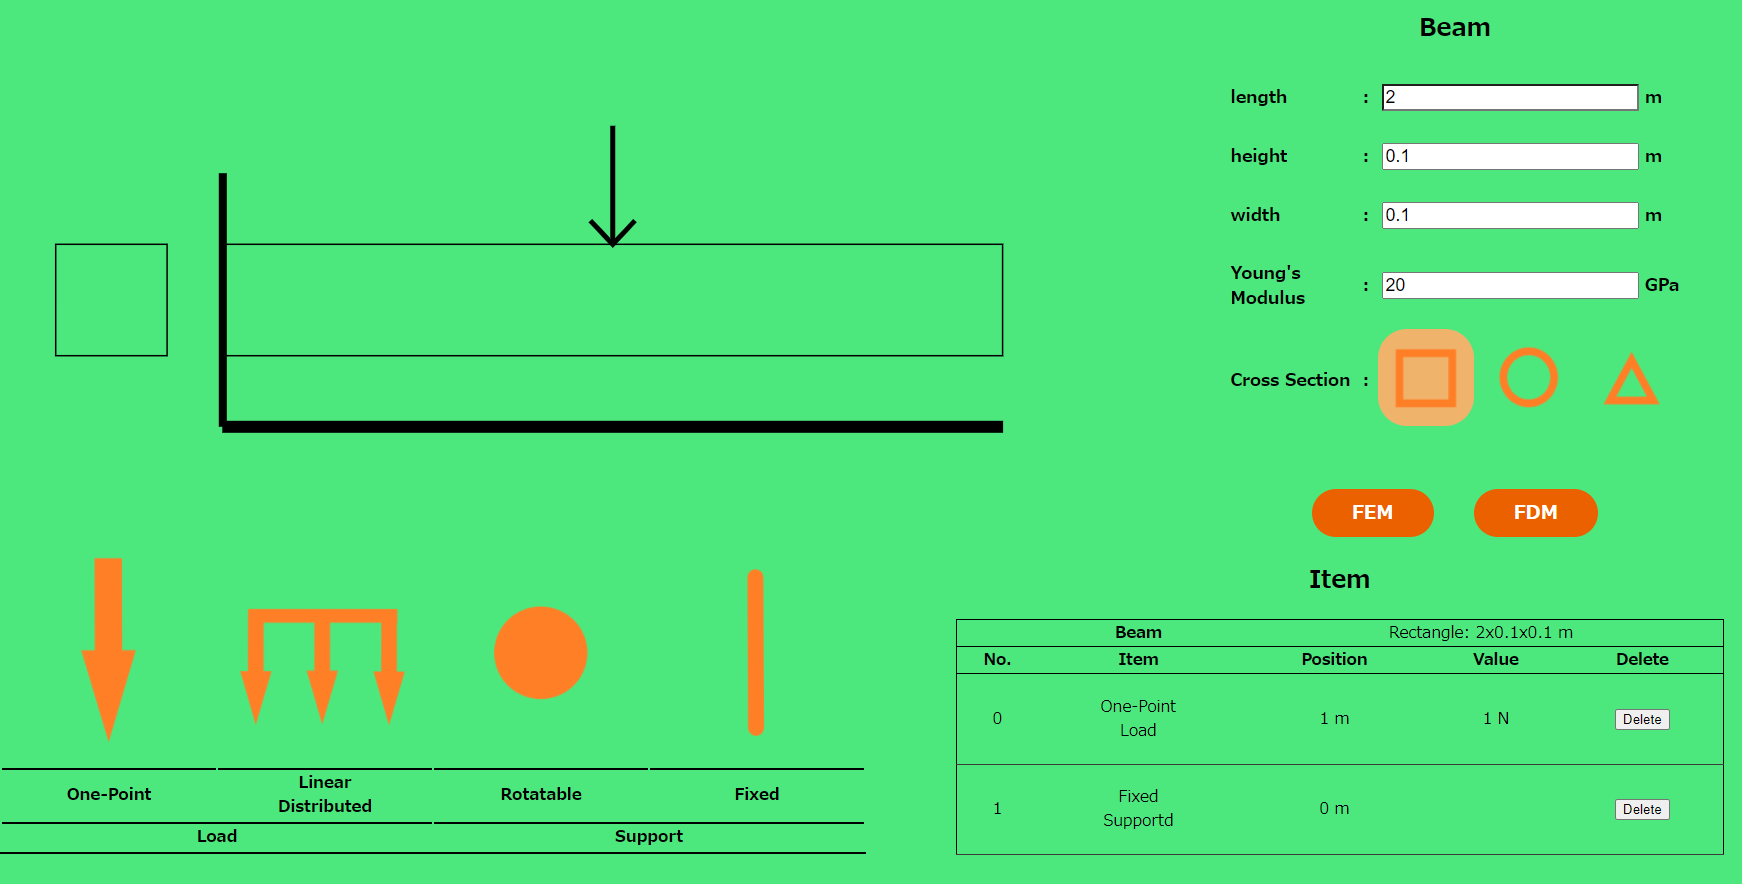
\includegraphics[width=13cm]{cantilever_one_model.PNG}
\caption{片持ち梁 一点荷重モデル}
\end{center}
\end{figure}

\subsubsection{解析解}

\begin{eqnarray*}
V &=& \left\{ \begin{array}{ll}
    W & (0\leq x<\frac{l}{2}) \\
    0 & (\frac{l}{2}\leq x < l)
  \end{array} \right. \\
M &=& \left\{ \begin{array}{ll}
    W\left(x-\frac{l}{2}\right) & (0\leq x<\frac{l}{2}) \\
    0 & (\frac{l}{2}\leq x < l)
  \end{array} \right. \\
\theta &=& \left\{ \begin{array}{ll}
    -\frac{W}{EI}\left(\frac{x^2}{2}-\frac{l}{2}x^2\right) & (0\leq x<\frac{l}{2}) \\
    \frac{Wl^2}{8EI} & (\frac{l}{2}\leq x < l)
  \end{array} \right. \\
w &=& \left\{ \begin{array}{ll}
    \frac{W}{EI}\left(\frac{x^3}{6}-\frac{l}{4}x^2\right) & (0\leq x<\frac{l}{2}) \\
    -\frac{W}{48EI}\left(6x-l\right) & (\frac{l}{2}\leq x < l)
  \end{array} \right.
\end{eqnarray*}

今回はモデルに示されているように, $l=2$ [m], $W=1$ [N], $E=20$ [GPa], $I=8.33\times10^{-6}$ [m$^4$]を用いる. これらの値を代入することで得られる解析解は以下のようになる(MATLABによる計算).

\begin{figure}[H]
\begin{center}
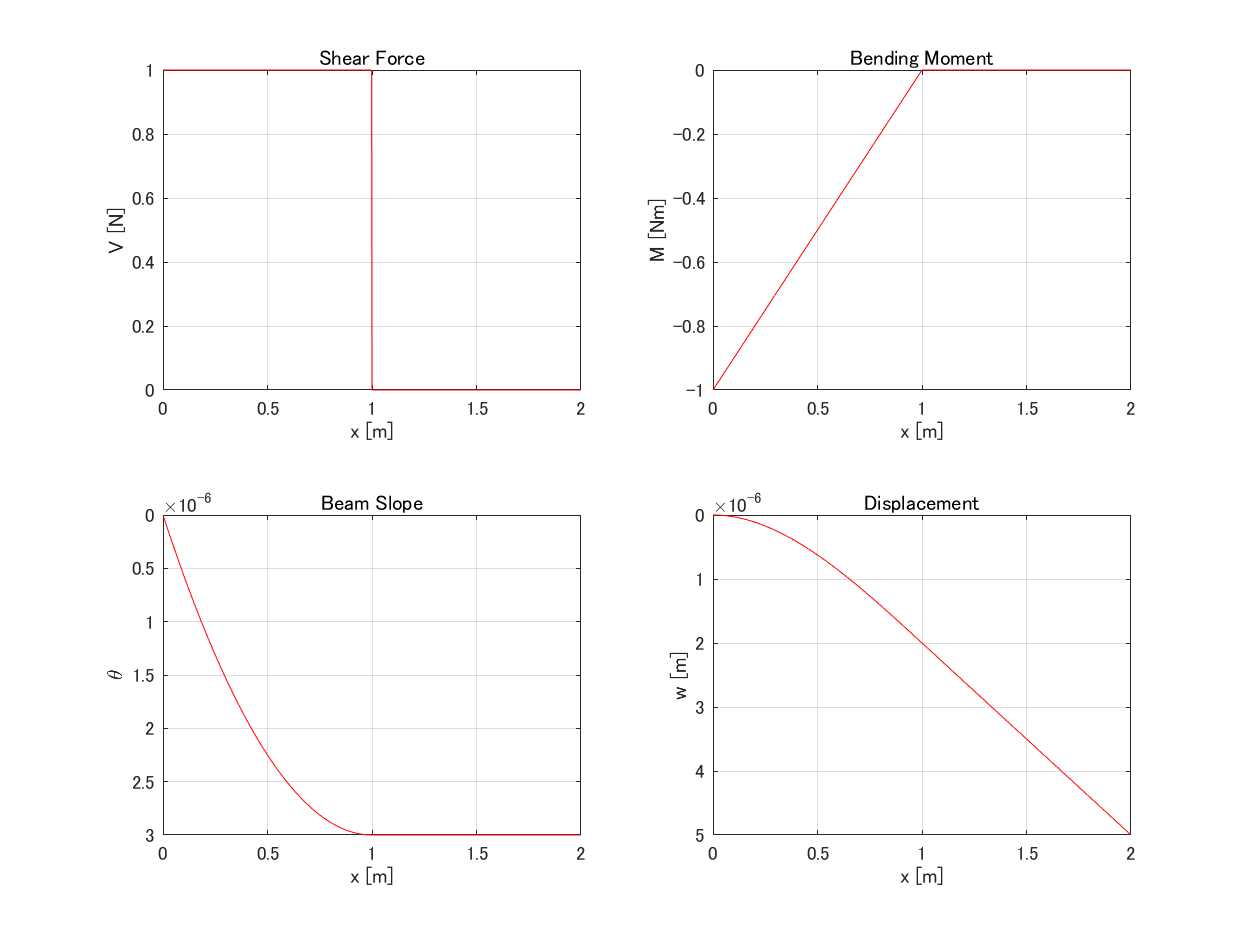
\includegraphics[width=10cm]{Cantilever_One_Beam.png}
\caption{片持ち梁 一点荷重 解析解}
\end{center}
\end{figure}

\subsubsection{シミュレーション結果}
\begin{table}[H]
\begin{center}
\caption{片持ち梁 一点荷重モデル シミュレーション結果の比較}
\begin{tabular}{|c|c|c|}
\hline
 & FEM & FDM \\
\hline
\hline
$V$ &
\begin{minipage}{6truecm}
\centering
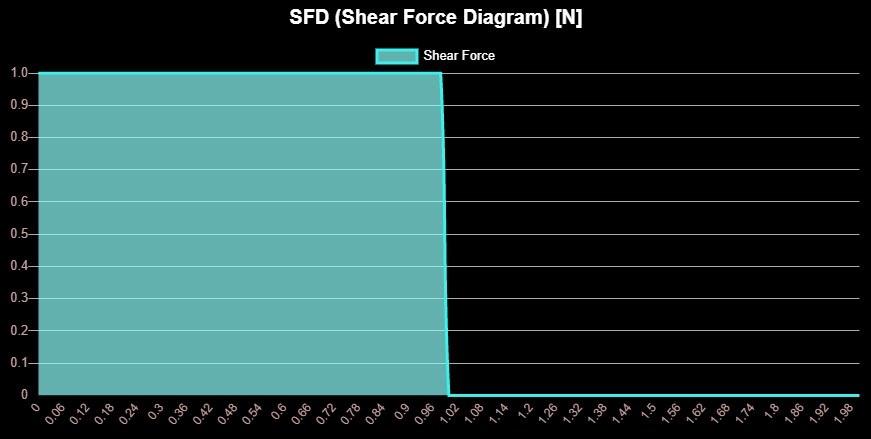
\includegraphics[width=6truecm]{cantilever_one_model_FEM_sf.PNG}
\end{minipage}
&
\begin{minipage}{6truecm}
\centering
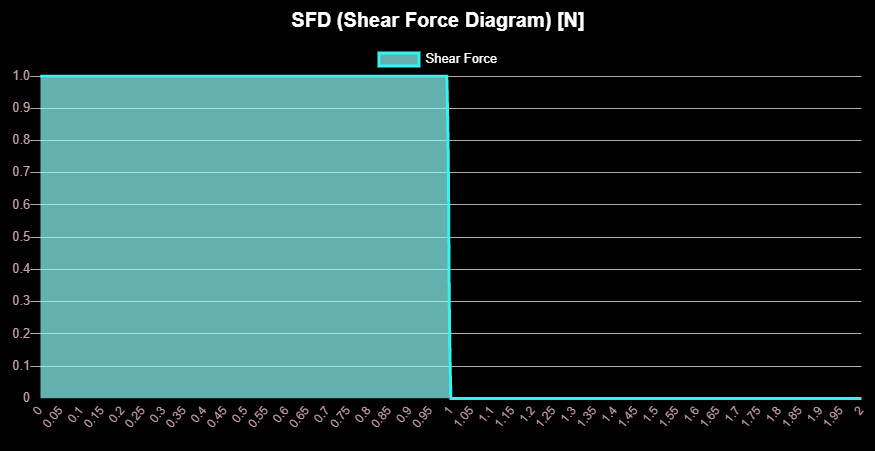
\includegraphics[width=6truecm]{cantilever_one_model_FDM_sf.PNG}
\end{minipage}
\\
\hline
$M$ &
\begin{minipage}{6truecm}
\centering
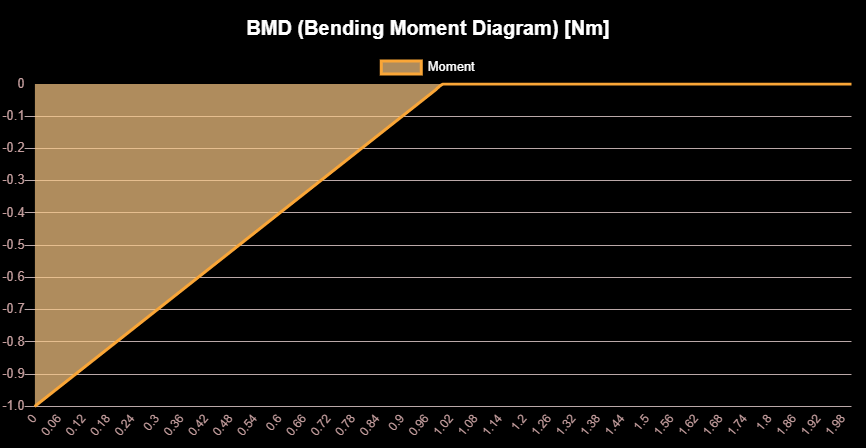
\includegraphics[width=6cm]{cantilever_one_model_FEM_bm.PNG}
\end{minipage}
&
\begin{minipage}{6truecm}
\centering
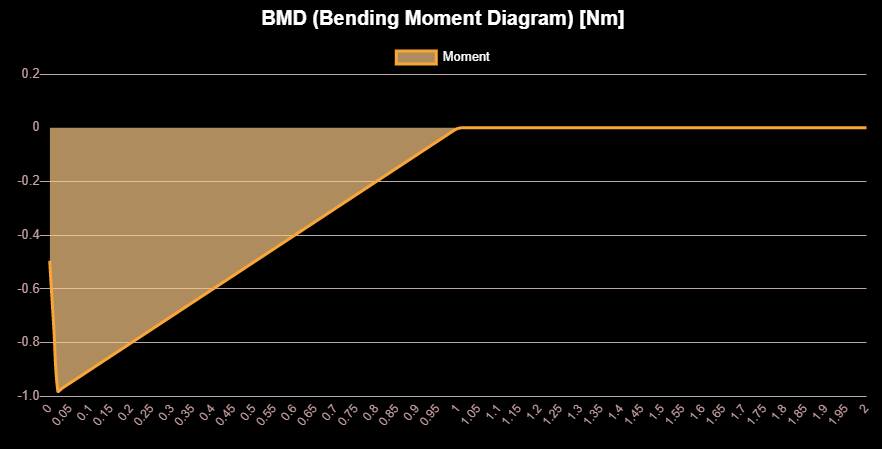
\includegraphics[width=6cm]{cantilever_one_model_FDM_bm.PNG}
\end{minipage}
\\
\hline
$\theta$ &
\begin{minipage}{6truecm}
\centering
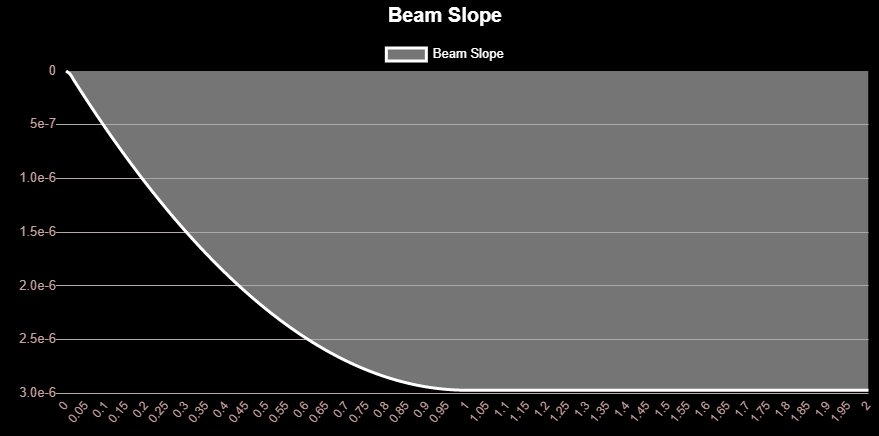
\includegraphics[width=6cm]{cantilever_one_model_FEM_slo.PNG}
\end{minipage}
&
\begin{minipage}{6truecm}
\centering
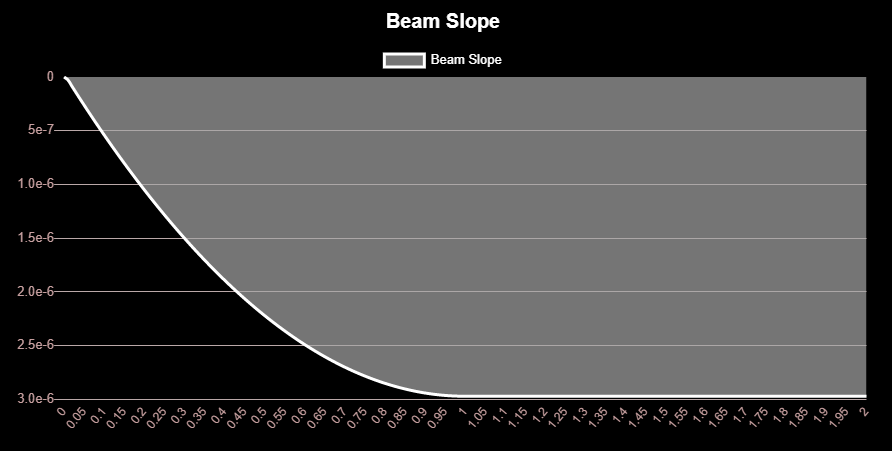
\includegraphics[width=6cm]{cantilever_one_model_FDM_slo.PNG}
\end{minipage}
\\
\hline
$w$ &
\begin{minipage}{6truecm}
\centering
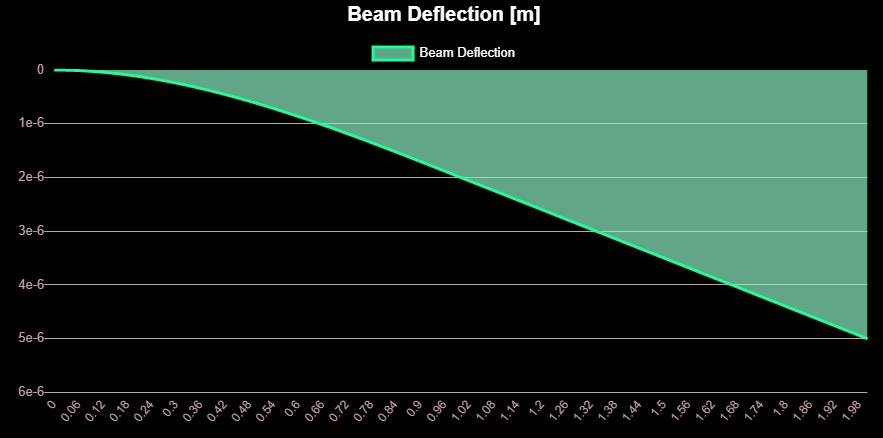
\includegraphics[width=6cm]{cantilever_one_model_FEM_def.PNG}
\end{minipage}
&
\begin{minipage}{6truecm}
\centering
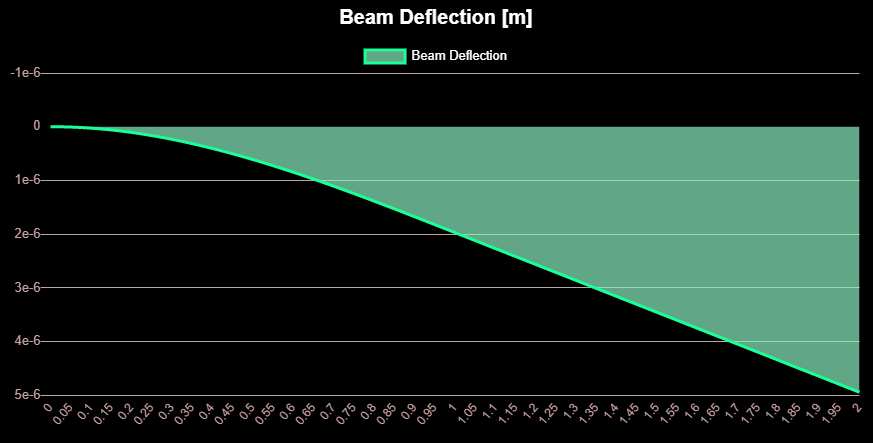
\includegraphics[width=6cm]{cantilever_one_model_FDM_def.PNG}
\end{minipage}
\\
\hline
\end{tabular}
\end{center}
\end{table}

\newpage
\subsection{分布荷重}
\subsubsection{モデル}
\begin{figure}[H]
\begin{center}
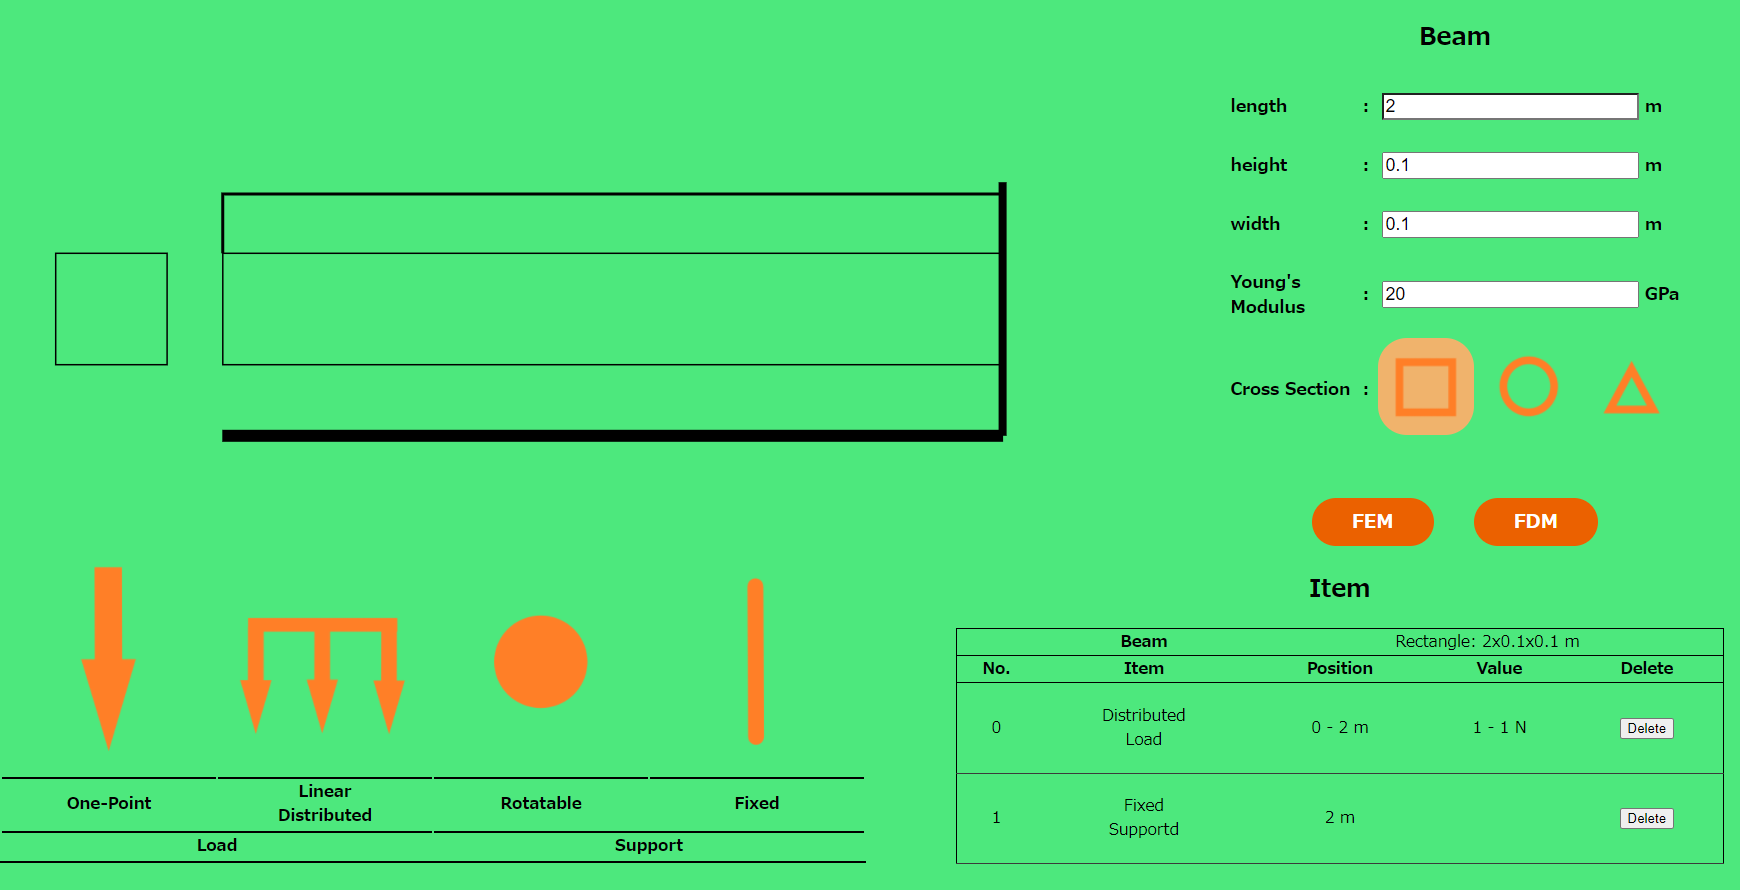
\includegraphics[width=13cm]{cantilever_distributed_model.PNG}
\caption{片持ち梁 分布荷重モデル}
\end{center}
\end{figure}

\subsubsection{解析解}
\begin{eqnarray*}
V &=& -Wx \\
M &=& -\frac{W}{2}x^2 \\
\theta &=& -\frac{W}{6EI}\left(x^3-l^3\right) \\
w &=& -\frac{W}{12EI}\left(x^4-4l^3x+3l^4\right)
\end{eqnarray*}
今回もモデルに示されているように, $l=2$ [m], $W=1$ [N], $E=20$ [GPa], $I=8.33\times10^{-6}$ [m$^4$]を用いる. これらの値を代入することで得られる解析解は以下のようになる(MATLABによる計算).

\begin{figure}[H]
\begin{center}
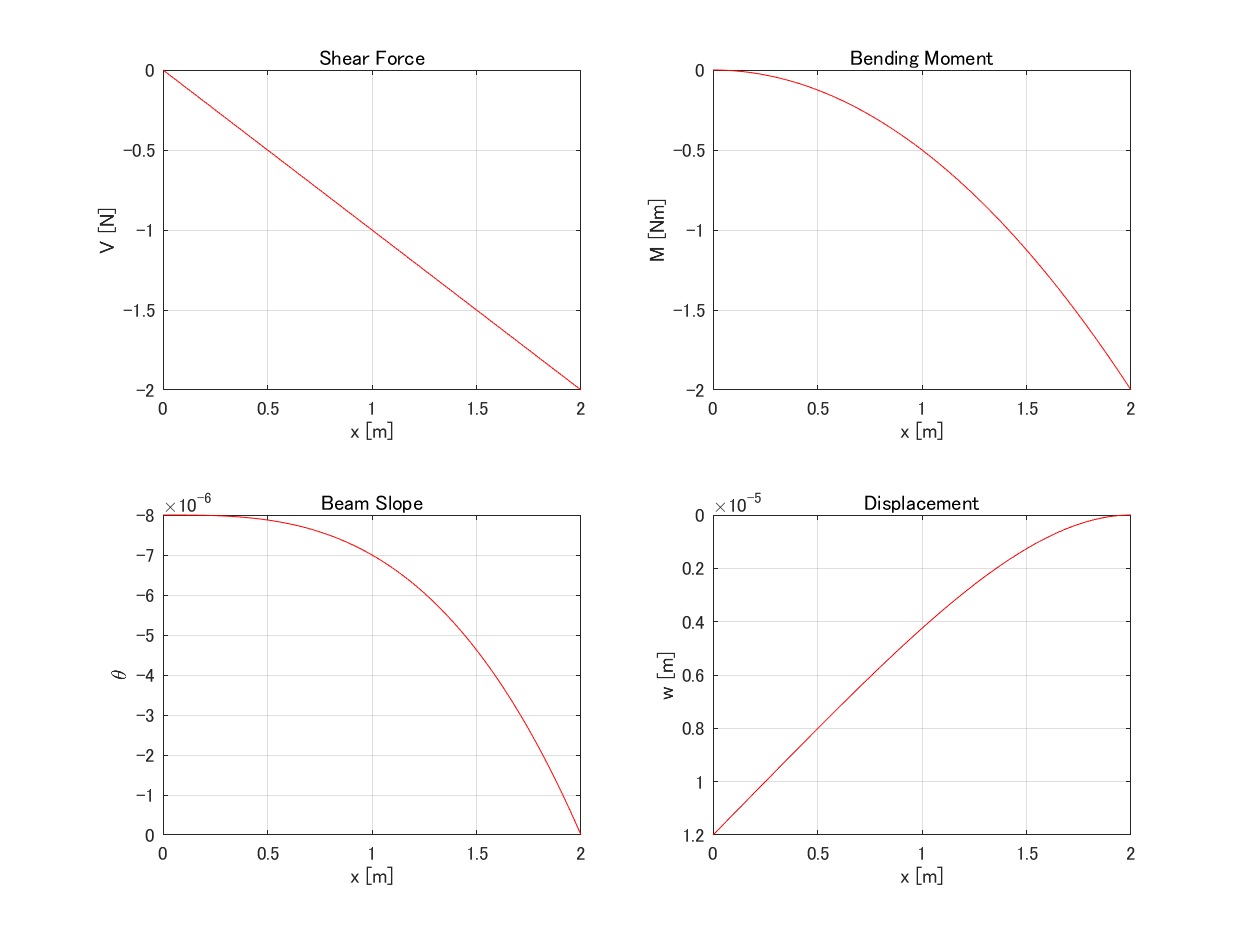
\includegraphics[width=10cm]{Cantilever_Distributed_Beam.png}
\caption{片持ち梁 分布荷重 解析解}
\end{center}
\end{figure}


\subsubsection{シミュレーション結果}
\begin{table}[H]
\begin{center}
\caption{片持ち梁 分布荷重モデル シミュレーション結果の比較}
\begin{tabular}{|c|c|c|}
\hline
 & FEM & FDM \\
\hline
\hline
$V$ &
\begin{minipage}{6truecm}
\centering
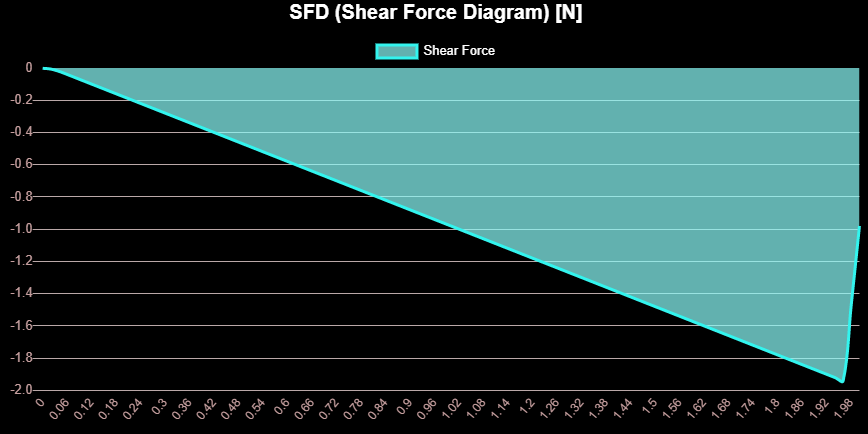
\includegraphics[width=6truecm]{cantilever_distributed_model_FEM_sf.PNG}
\end{minipage}
&
\begin{minipage}{6truecm}
\centering
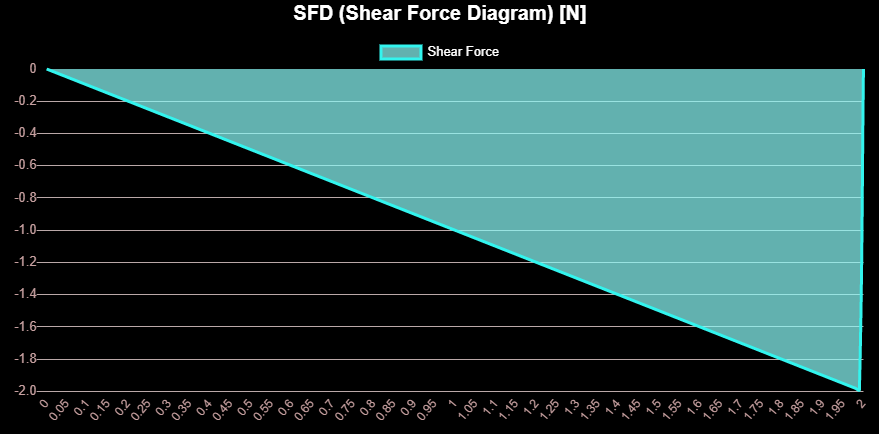
\includegraphics[width=6truecm]{cantilever_distributed_model_FDM_sf.PNG}
\end{minipage}
\\
\hline
$M$ &
\begin{minipage}{6truecm}
\centering
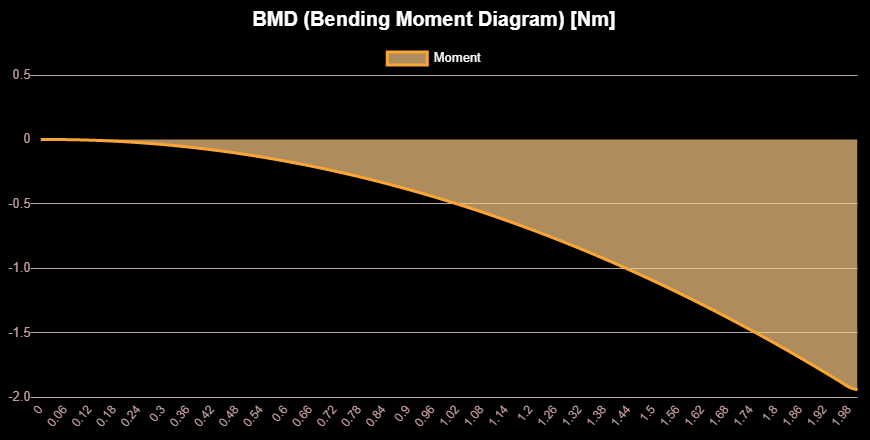
\includegraphics[width=6cm]{cantilever_distributed_model_FEM_bm.PNG}
\end{minipage}
&
\begin{minipage}{6truecm}
\centering
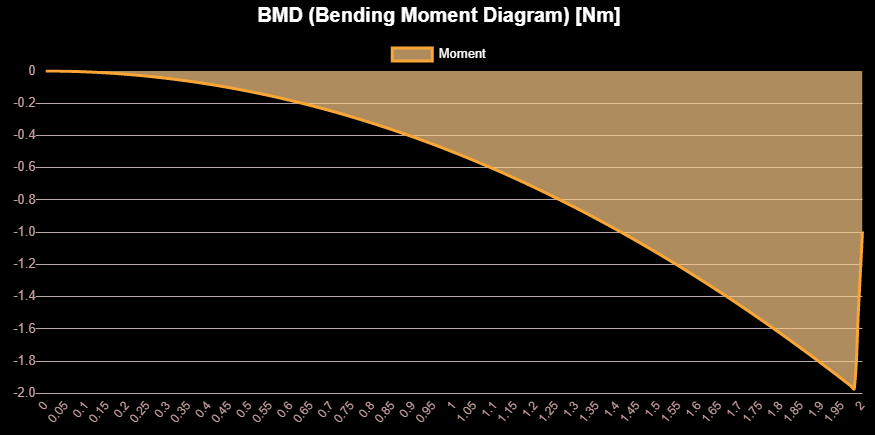
\includegraphics[width=6cm]{cantilever_distributed_model_FDM_bm.PNG}
\end{minipage}
\\
\hline
$\theta$ &
\begin{minipage}{6truecm}
\centering
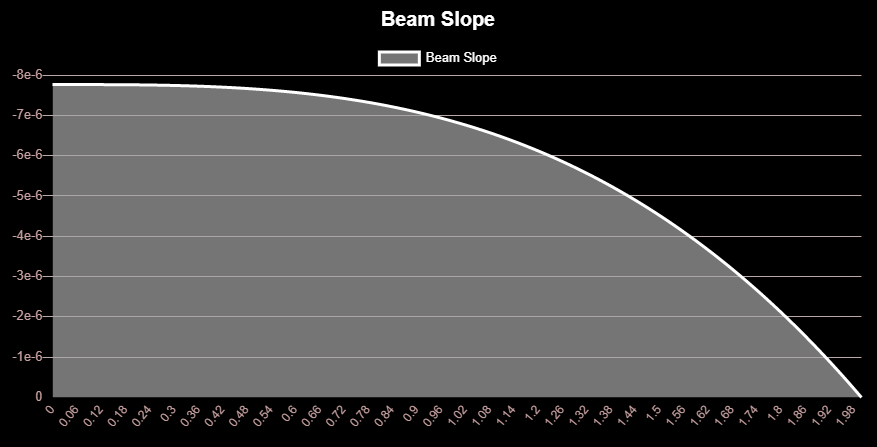
\includegraphics[width=6cm]{cantilever_distributed_model_FEM_slo.PNG}
\end{minipage}
&
\begin{minipage}{6truecm}
\centering
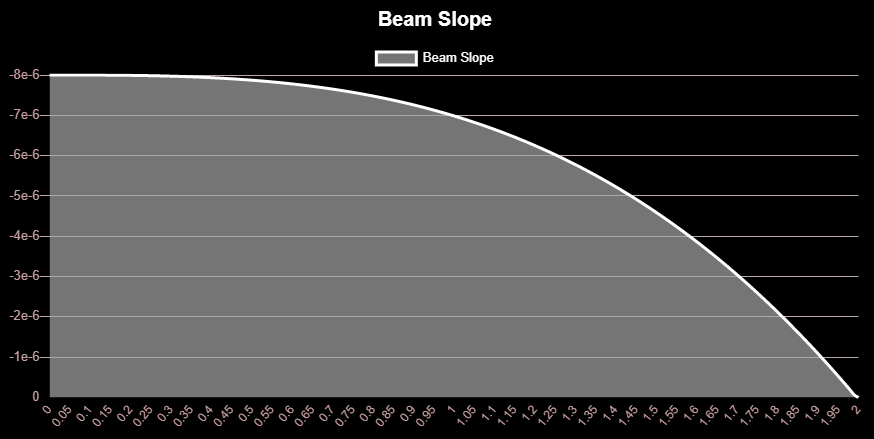
\includegraphics[width=6cm]{cantilever_distributed_model_FDM_slo.PNG}
\end{minipage}
\\
\hline
$w$ &
\begin{minipage}{6truecm}
\centering
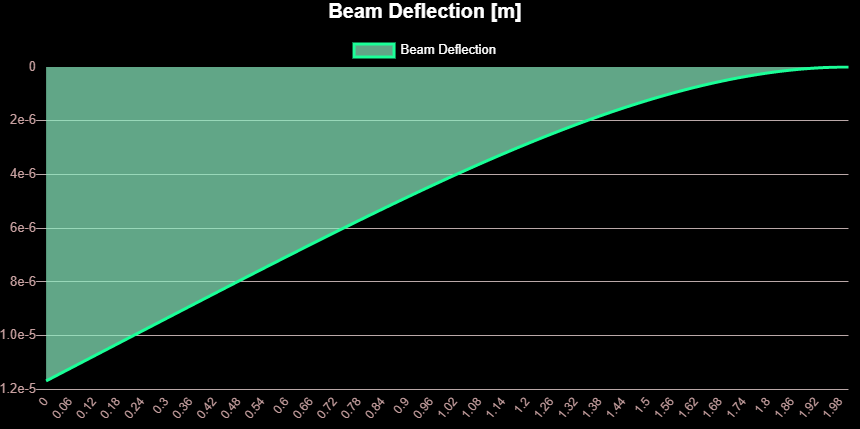
\includegraphics[width=6cm]{cantilever_distributed_model_FEM_def.PNG}
\end{minipage}
&
\begin{minipage}{6truecm}
\centering
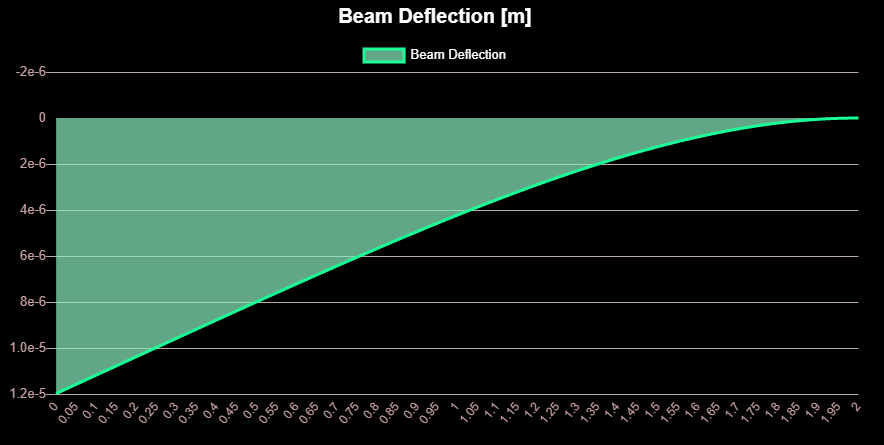
\includegraphics[width=6cm]{cantilever_distributed_model_FDM_def.PNG}
\end{minipage}
\\
\hline
\end{tabular}
\end{center}
\end{table}

\newpage
\part{シミュレーション (不静定梁問題)}
ここまでのシミュレーション例では, 解析解を簡単に求めることができる静定梁問題について扱った, しかし, このシミュレータでは数値解析手法を用いてるため, 不静定梁問題も解くことが可能である. ここからは, 不静定梁問題のシミュレーション例を紹介する.

\newpage
\section{両端固定梁}
\subsection{一点荷重}
\subsubsection{モデル}
\begin{figure}[H]
\begin{center}
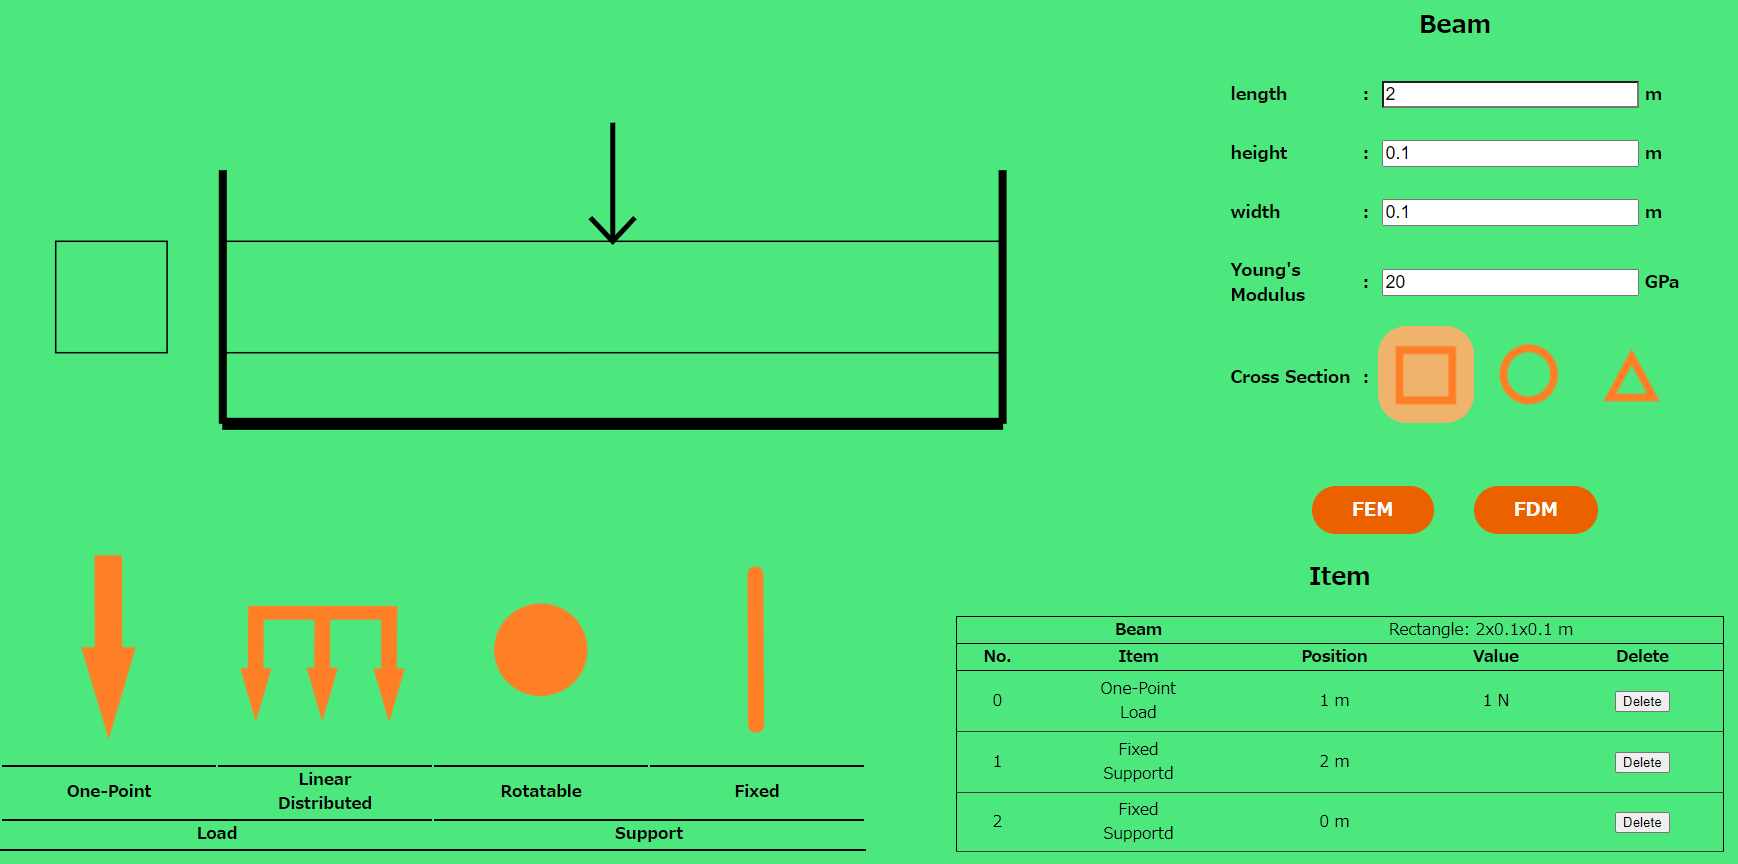
\includegraphics[width=11cm]{fixed_one_model.PNG}
\caption{両端固定梁 一点荷重モデル}
\end{center}
\end{figure}


\subsubsection{シミュレーション結果}
\begin{table}[H]
\begin{center}
\caption{両端固定梁 一点荷重モデル シミュレーション結果の比較}
\begin{tabular}{|c|c|c|}
\hline
 & FEM & FDM \\
\hline
\hline
$V$ &
\begin{minipage}{6truecm}
\centering
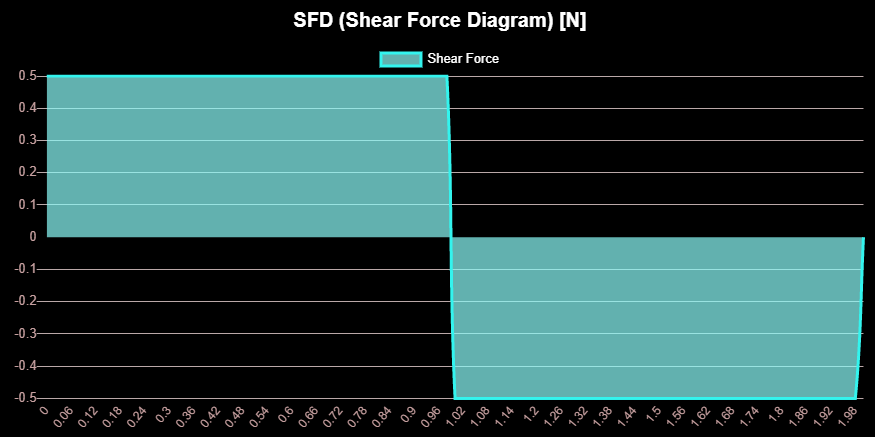
\includegraphics[width=6truecm]{fixed_one_model_FEM_sf.PNG}
\end{minipage}
&
\begin{minipage}{6truecm}
\centering
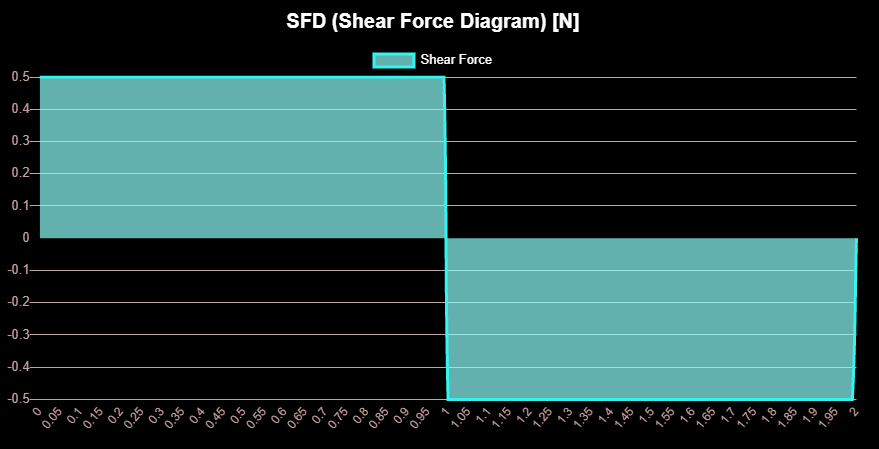
\includegraphics[width=6truecm]{fixed_one_model_FDM_sf.PNG}
\end{minipage}
\\
\hline
$M$ &
\begin{minipage}{6truecm}
\centering
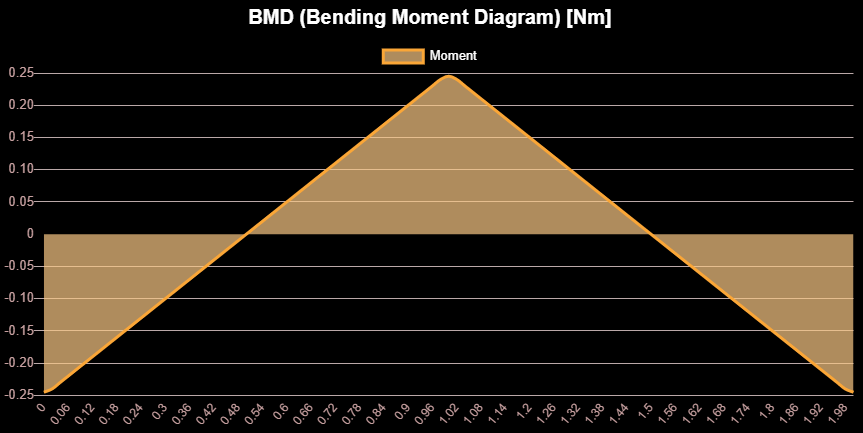
\includegraphics[width=6cm]{fixed_one_model_FEM_bm.PNG}
\end{minipage}
&
\begin{minipage}{6truecm}
\centering
\includegraphics[width=6cm]{fixed_one_model_FDM_bm.PNG}
\end{minipage}
\\
\hline
$\theta$ &
\begin{minipage}{6truecm}
\centering
\includegraphics[width=6cm]{fixed_one_model_FEM_slo.PNG}
\end{minipage}
&
\begin{minipage}{6truecm}
\centering
\includegraphics[width=6cm]{fixed_one_model_FDM_slo.PNG}
\end{minipage}
\\
\hline
$w$ &
\begin{minipage}{6truecm}
\centering
\includegraphics[width=6cm]{fixed_one_model_FEM_def.PNG}
\end{minipage}
&
\begin{minipage}{6truecm}
\centering
\includegraphics[width=6cm]{fixed_one_model_FDM_def.PNG}
\end{minipage}
\\
\hline
\end{tabular}
\end{center}
\end{table}

\newpage
\subsection{分布荷重}
\subsubsection{モデル}

\begin{figure}[H]
\begin{center}
\includegraphics[width=11cm]{fixed_distributed_model.PNG}
\caption{両端固定梁 分布荷重モデル}
\end{center}
\end{figure}


\subsubsection{シミュレーション結果}
\begin{table}[H]
\begin{center}
\caption{両端固定梁 分布荷重モデル シミュレーション結果の比較}
\begin{tabular}{|c|c|c|}
\hline
 & FEM & FDM \\
\hline
\hline
$V$ &
\begin{minipage}{6truecm}
\centering
\includegraphics[width=6truecm]{fixed_distributed_model_FEM_sf.PNG}
\end{minipage}
&
\begin{minipage}{6truecm}
\centering
\includegraphics[width=6truecm]{fixed_distributed_model_FDM_sf.PNG}
\end{minipage}
\\
\hline
$M$ &
\begin{minipage}{6truecm}
\centering
\includegraphics[width=6cm]{fixed_distributed_model_FEM_bm.PNG}
\end{minipage}
&
\begin{minipage}{6truecm}
\centering
\includegraphics[width=6cm]{fixed_distributed_model_FDM_bm.PNG}
\end{minipage}
\\
\hline
$\theta$ &
\begin{minipage}{6truecm}
\centering
\includegraphics[width=6cm]{fixed_distributed_model_FEM_slo.PNG}
\end{minipage}
&
\begin{minipage}{6truecm}
\centering
\includegraphics[width=6cm]{fixed_distributed_model_FDM_slo.PNG}
\end{minipage}
\\
\hline
$w$ &
\begin{minipage}{6truecm}
\centering
\includegraphics[width=6cm]{fixed_distributed_model_FEM_def.PNG}
\end{minipage}
&
\begin{minipage}{6truecm}
\centering
\includegraphics[width=6cm]{fixed_distributed_model_FDM_def.PNG}
\end{minipage}
\\
\hline
\end{tabular}
\end{center}
\end{table}

\newpage

\section{3点支持問題}
ここまでのシミュレーションでは間違いなく, 解析解と比較しても正しい結果が得られていた. しかし, 入力するデータによっては問題が起こる可能性がある. その例を以下で紹介します. 今回は回転支持点3つで支えられる梁に一点荷重を与えた以下のモデルについて考える. 

\begin{figure}[H]
\begin{center}
\includegraphics[width=11cm]{three_model.PNG}
\caption{3点支持モデル}
\end{center}
\end{figure}

そして, この梁のシミュレーション結果は, FDMおよびFEMの両方において以下のようになる.

\begin{figure}[H]
\begin{center}
\includegraphics[width=13cm]{three_model_result.PNG}
\caption{3点支持シミュレーション結果}
\end{center}
\end{figure}

ここで, 今回のシミュレーションでは, 仮定により自重を考慮していない. そのため, 一番右の回転支持点では梁を支持しない結果となることが予想される. しかし, このシミュレーションでは支持点での境界条件の優先度を高くしているため, このような結果になっている. この場合は, 考慮する対象を左半分の単純支持梁の身を考えるなど代替案を考慮していただく必要がある.

このように, このシミュレータの結果には間違いが起ることがあるため, FEMやFDMの結果を比較したり, 考慮している状況について深く考察することが必要になる.


\newpage
\part{参考文献}
\begin{itemize}
\item[[1]] 岩熊哲夫 小山茂著, 構造と連続体の力学基礎, \url{http://mechanics.civil.tohoku.ac.jp/bear/n2.pdf}
\item[[2]] 市川昌弘 江藤元大 船見国男 本間恭二共著, 材料力学, 技報堂出版, 2016
\end{itemize}


\end{document}
